\documentclass[12pt,a4paper]{article}

% Language setting
\usepackage[british]{babel}

% Set page size and margins
\usepackage[a4paper,top=2cm,bottom=2cm,left=2.5cm,right=2.5cm,marginparwidth=1.75cm]{geometry}

%----------- APA style references & citations (starting) ---
% Useful packages
%\usepackage[natbibapa]{apacite} % APA-style citations.

\usepackage[bibstyle=numeric, sorting=nyt, maxnames=99,minnames=1, giveninits=true, abbreviate=true, backend=bibtex]{biblatex} % APA 7th edition style citations using biblatex
\addbibresource{references.bib} % Your .bib file

% Formatting DOI in APA-7 style
%\renewcommand{\doiprefix}{https://doi.org/}

% Add additional APA 7th edition requirements
%\DeclareLanguageMapping{british}{british-apa} % Set language mapping
%\DeclareFieldFormat[article]{volume}{\apanum{#1}} % Format volume number

\DeclareFieldFormat[article]{title}{#1,}
\DeclareFieldFormat[inproceedings]{title}{#1,}
\DeclareFieldFormat[book]{title}{#1,}
% 调整作者和标题之间的分隔符为逗号
\renewcommand*{\newunitpunct}{\addcomma\space}

\AtEveryBibitem{\clearfield{number}}
\renewbibmacro{in:}{} 
\DeclareFieldFormat{pages}{#1}
\renewbibmacro*{journal+issuetitle}{%
  \iffieldundef{shortjournal}%
    {\usebibmacro{journal}}% 如果 shortjournal 未定义,使用 journal
    {\mkbibemph{\printfield{shortjournal}}}% 否则只使用 shortjournal
  \setunit{\addspace}%
  \usebibmacro{volume+number+eid}%
  \setunit*{\addspace}% 在 journal 和 volume 之间用空格
  \setunit{\addcolon\space}%
  \newunit}


\DeclareFieldFormat[article]{volume}{\mkbibbold{#1}} % 将 volume 加粗
\DeclareFieldFormat[article]{year}{(#1)} % 确保 year 格式正常

\renewbibmacro*{volume+number+eid}{%
  \printfield{volume}% 打印加粗的 volume
  \setunit*{\addspace}% 用空格分隔 volume 和 year
  \printfield{year}% 打印年份
  \setunit{\addspace}% 年份后空格
  \printfield{number}%
  \setunit{\addcomma\space}% 如果有 number,加逗号和空格
  \printfield{eid}}


\DeclareFieldFormat[book]{title}{\mkbibemph{#1}}
\DeclareFieldFormat{publisher}{#1}
\DeclareFieldFormat{address}{#1}
\renewbibmacro*{publisher+location+date}{%
  \iflistundef{publisher}
    {}
    {\addcomma\space\printlist{publisher}}%
  \iflistundef{location}
    {}
    {\addcomma\space\printlist{location}}%
  \setunit*{\addcomma\space}%
  \printfield{year}%
}


% Modify 'and' to '&' in the bibliography
%\renewcommand*{\finalnamedelim}{%
%\ifnumgreater{\value{liststop}}{2}{\finalandcomma}{}%
%\addspace\&\space}
  
%----------- APA style references & citations (ending) ---


\usepackage{amsthm}  % 需要包含amsthm宏包

\newtheorem{definition}{Definition}  % 定义Definition环境
\newtheorem{theorem}{Theorem}  
\newtheorem{lemma}{Lemma} 
\newtheorem{remark}{Remark} 
\newtheorem{example}{Example} 
\newtheorem{proposition}{Proposition}


\usepackage{amsmath}
\numberwithin{equation}{section}  % 让公式编号按章节计数
\usepackage{graphicx}
\usepackage{subcaption} 
\usepackage{tikz}
\usepackage[colorlinks=true, allcolors=blue]{hyperref}
\usepackage{hyperref}
%\usepackage{orcidlink}
\usepackage[title]{appendix}
\usepackage{mathrsfs}
\usepackage{amsfonts}
\usepackage{booktabs} % For \toprule, \midrule, \botrule
\usepackage{caption}  % For \caption
\usepackage{threeparttable} % For table footnotes
\usepackage[linesnumbered,ruled,vlined]{algorithm2e}
\usepackage{algpseudocode}  % For defining algorithms with pseudocode
\usepackage{algorithmicx}
\usepackage{algpseudocode}
\usepackage{listings}
\usepackage{enumitem}
\usepackage{chngcntr}
\usepackage{booktabs}
\usepackage{lipsum}
\usepackage{subcaption}
\usepackage{authblk}
\usepackage[T1]{fontenc}    % Font encoding
\usepackage{csquotes}       % Include csquotes
\usepackage{diagbox}
\usepackage{xcolor}


\usepackage{stmaryrd}
%\usepackage{fourier}


\newcommand{\vb}{\boldsymbol{v}}
\newcommand{\wb}{\boldsymbol{w}}
\newcommand{\ub}{\boldsymbol{u}}
\newcommand{\Hb}{\boldsymbol{H}}
\newcommand{\curlb}{\mathbf{curl}}
\newcommand{\Lb}{\boldsymbol{L}}
\newcommand{\Vb}{\boldsymbol{V}}
\newcommand{\Eb}{\boldsymbol{E}}
\newcommand{\Bb}{\boldsymbol{B}}
\newcommand{\nb}{\boldsymbol{n}}
\newcommand{\Jb}{\boldsymbol{J}}
\newcommand{\lb}{\boldsymbol{l}}
\newcommand{\xb}{\boldsymbol{x}}
\newcommand{\xib}{\boldsymbol{\xi}}
\newcommand{\etab}{\boldsymbol{\eta}}
\newcommand{\Cb}{\boldsymbol{C}}
\newcommand{\fb}{\boldsymbol{f}}
\newcommand{\zerob}{\boldsymbol{0}}
\newcommand{\Hcurlb}{\textbf{\textit{H}(curl)}}
\newcommand{\varPsib}{\boldsymbol{\varPsi}}
\newcommand{\zetab}{\boldsymbol{\zeta}}
\newcommand{\qb}{\boldsymbol{q}}
\newcommand{\pb}{\boldsymbol{p}}
\newcommand{\Pib}{\boldsymbol{\Pi}}


% Customize line spacing
\usepackage{setspace}
\onehalfspacing % 1.5 line spacing

% Redefine section and subsection numbering format
\usepackage{titlesec}
\titleformat{\section} % Redefine section numbering format
  {\normalfont\Large\bfseries}{\thesection.}{1em}{}
  
% Customize line numbering format to right-align line numbers
\usepackage{lineno} % Add the lineno package
\renewcommand\linenumberfont{\normalfont\scriptsize\sffamily\color{blue}}
\rightlinenumbers % Right-align line numbers

%\linenumbers % Enable line numbering

% Define a new command for the fourth-level title.
\newcommand{\subsubsubsection}[1]{%
  \vspace{\baselineskip}% Add some space
  \noindent\textbf{#1\\}\quad% Adjust formatting as needed
}
% Change the position of the table caption above the table
\usepackage{float}   % for customizing caption position
\usepackage{caption} % for customizing caption format
\captionsetup[table]{position=top} % caption position for tables

% Define the unnumbered list
\makeatletter
\newenvironment{unlist}{%
  \begin{list}{}{%
    \setlength{\labelwidth}{0pt}%
    \setlength{\labelsep}{0pt}%
    \setlength{\leftmargin}{2em}%
    \setlength{\itemindent}{-2em}%
    \setlength{\topsep}{\medskipamount}%
    \setlength{\itemsep}{3pt}%
  }%
}{%
  \end{list}%
}
\makeatother

% Suppress the warning about \@parboxrestore
\pdfsuppresswarningpagegroup=1


%-------------------------------------------
% Paper Head
%-------------------------------------------
\title{A Discontinuous Galerkin Method for \Hcurlb-Elliptic Hemivariational Inequalities}

\author[1,2,3]{Xiajie Huang\thanks{Email: \texttt{xj.huang@sjtu.edu.cn}}}

\author[1]{Fei Wang\thanks{The work of this author was partially supported by
			the National Natural Science Foundation of China (Grant No.\ 12171383). Email: \texttt{feiwang.xjtu@xjtu.edu.cn}}}
\author[4]{Weimin Han\thanks{The work of this author was partially supported by Simons Foundation Collaboration Grants (Grant No.\ 850737). Email: \texttt{weimin-han@uiowa.edu}}}
\author[5]{Min Ling \thanks{Email: \texttt{lingmin@imu.edu.cn}}}
%\author[3]{Fourth Author}
%\author[1,*]{Fifth Author}
\affil[1]{\small School of Mathematics and Statistics, Xi’an Jiaotong University, Xi’an, Shaanxi 710049, China}
\affil[2]{\small School of Mathematical Sciences, Shanghai Jiao Tong University, Shanghai 200240, China}
\affil[3]{Shanghai Artificial Intelligence Laboratory, Shanghai, China}
\affil[4]{Department of Mathematics, University of Iowa, Iowa City, IA 52242, USA}
\affil[5]{School of Mathematical Sciences, Inner Mongolia University, Hohhot, 010021, China}
%\affil[*]{Corresponding author: \texttt{user\_id@university.edu}}

\date{}  % Remove date

\begin{document}
\maketitle

\begin{abstract}  
%Due to widespread applications, research on high-temperature superconductors is always at the forefront of physics research.
%In 1962, C. P. Bean proposed a critical state model to describe high-temperature superconductors\textsuperscript{\cite{bean1964magnetization,bean1962magnetization}}. Han et al. extended it to a general non-monotonic case in their paper \cite{han2022numerical} and obtained a $\Hcurlb$-elliptic hemivariational inequality through a temporal semi-discretization. 

In this paper, we develop a Discontinuous Galerkin (DG) method for solving $\Hcurlb$-elliptic hemivariational inequalities. By selecting an appropriate numerical flux, we construct an  Interior Penalty Discontinuous Galerkin (IPDG) scheme. A comprehensive numerical analysis of the IPDG method is conducted, addressing key aspects such as consistency, boundedness, stability, and the existence, uniqueness, uniform boundedness of the numerical solutions. Building on these properties, we establish a priori error estimates, demonstrating the optimal convergence order of the numerical solutions under suitable solution regularity assumptions. Finally, a numerical example is presented to illustrate the theoretically predicted convergence order and to show the effectiveness of the proposed method.
  
\end{abstract}

%\textbf{Keywords}: keyword1, keyword2, keyword3, keyword4, keyword5, keyword6.  

%-------------------------------------------
% Paper Body
%-------------------------------------------
%--- Section ---%
%\section*{Nomenclature}

%\begin{tabbing}
%$T$\qquad \= Temperature (K)\\
%$u_i$ \> Velocity in the x-direction (m/s)\\
%$\tau_{ij}$ \> Shear stress (N/m2)\\
%$\omega$ \> Specific turbulent dissipation rate (1/s)\\
%$Y_\omega$ \> Dissipation of $\omega$
%\end{tabbing}
\textbf{Keywords}: Discontinuous Galerkin method; \Hcurlb-elliptic hemivariational inequality; non-monotonicity; high-temperature superconductors; error estimates



%--- Section ---%
\section{Introduction}

To describe the mixed state of high-temperature superconductors, C. P. Bean proposed the critical state theory of high-temperature superconductors \textsuperscript{\cite{bean1964magnetization,bean1962magnetization}}. The basic idea of this model can be described as follows. When a superconductor is in the mixed state, the magnitude of the current density $|\Jb|$ cannot exceed a critical value $g$. In the regions penetrated by the magnetic field, the current density is $|\Jb| = g$, and the electric field $\Eb$ is parallel to the current. When the magnitude of the current density $\Jb$ is strictly less than the critical value $g$, the electric field $\Eb = \zerob$. Mathematically, this can be expressed as
\begin{equation*}
|\Jb| \leq g; \quad |\Jb| < g \Rightarrow \Eb = \zerob; \quad |\Jb| = g \Rightarrow \Jb = \kappa \Eb \text{ for some } \kappa \geq 0,
\end{equation*}
One can eliminate the unknown parameter $\kappa$ and derive the following equivalent expression:
 \begin{equation}\label{eqn1.0}
 	|\Jb|\leq g, \quad \Jb\cdot\Eb=g|\Eb|.
 \end{equation}
With the use of the notion of convex subdifferential $\partial_c$, the relation can be compactly written as
 \begin{equation}\label{current}
 	\Jb\in\partial_c(g|\Eb|).
 \end{equation}
 
The condition (\ref{current}) represents a non-smooth monotone relation; thus the mathematical models can be described by variational inequalities. The Maxwell system subject to the above Bean critical state model leads to Maxwell variational inequalities that have been analyzed theoretically and numerically in a number of papers, e.g., \cite{WY19, WYZ20, Yo20} and more recently, \cite{MWY24}. More generally, the critical current density $g$ may depend on the temperature and magnetic field strength, and it has been shown in \cite{daeumling1990oxygen, cantoni2005anisotropic} that the relationship between the critical current density and magnetic field strength is often non-monotonic. Variational inequalities cannot be used to describe such complex phenomena. In \cite{han2022numerical}, the condition (\ref{current}) is extended to the form
\begin{equation} \label{eqn.currentClarke}
\Jb \in \partial\psi(\Eb).
\end{equation}
The function $\psi(\xb, \Eb): \Omega \times \mathbb{R}^3 \rightarrow \mathbb{R}$ is locally Lipschitz continuous with respect to the variable $\Eb$ and this dependence is allowed to be non-convex. To simplify the notation, we write $\psi(\Eb)$ for $\psi(\xb, \Eb)$.  The symbol $\partial \psi(\Eb)$ denotes the Clarke subdifferential of $\psi$ with respect to the variable $\Eb$. With the use of the condition \eqref{eqn.currentClarke}, the mathematical model can be expressed as a hemivariational inequality (HVI).

Since an analytical solution to the HVI is generally not obtainable, it is crucial to develop numerical methods to solve HVIs. The reference \cite{haslinger1999finite} summarizes early results on the use of the finite element method (FEM) for solving HVI problems, including algorithms for obtaining numerical solutions and their convergence properties. Steady efforts have been devoted to development and analysis of numerical methods to solve various HVI problems. In \cite{barboteu2013analytical}, an elliptic hemivariational inequality is discussed numerically for a model of static bilateral frictional contact between linear elastic bodies. 
%, they tried to use finite element method to solve this problem and provides a suboptimal error estimate for the finite element numerical solution. 
References \cite{kalita2012regularity, Kalita2013Convergence} analyze the time semi-discrete scheme for the parabolic hemivariational inequality problem and reference \cite{kalita2014semidiscrete} extends the convergence results from \cite{Kalita2013Convergence} to the more general time-discrete $\theta$-scheme ($\theta\in (0,1]$).  
A class of variational-hemivariational inequalities is studied both theoretical and numerical analysis in \cite{MR3284570}, and for the first time an optimal first-order error estimate is presented for the linear finite element solution of HVIs.  Reference \cite{barboteu2015numerical} studies a spatial semi-discrete Galerkin approximation scheme and a fully discrete approximation scheme for a hyperbolic hemivariational inequality. Under appropriate solution regularity assumptions, optimal-order error estimates for the linear finite element solution of both schemes are provided. 
Later on, many studies have been conducted on the convergence theory and error estimates for the finite element numerical solution of variational-hemivariational inequalities, such as elliptic HVIs\textsuperscript{\cite{han2017numerical,han2018numerical,han2018numerical2}}, parabolic HVIs\textsuperscript{\cite{han2021numerical}}, hyperbolic HVIs\textsuperscript{\cite{barboteu2015numerical}}, history-dependent HVIs\textsuperscript{\cite{wang2020numerical, xu2019numerical, sofonea2015numerical, xu2019numerical2,ling2024numerical}}, Stokes HVIs\textsuperscript{\cite{fang2020finite}} and Navier-Stokes HVIs\textsuperscript{\cite{han2021mixed,jing2024finite,wang2024optimal}}. Summary accounts of recent development on the numerical analysis of variational-hemivariational inequalities can be found in \cite{han2019numerical, HFWH25}.

Recently, other numerical methods have also been studied to solve HVIs.  Conforming virtual element methods are used in \cite{feng2019virtual, feng2021virtual, wang2021virtual} to solve elliptic HVIs. Nonconforming virtual element methods are used in \cite{ling2020nonconforming, feng2022nonconforming} to solve HVI problems.  The Discontinuous Galerkin (DG) method is first applied in \cite{wang2020discontinuous} to solve elliptic HVIs for semi-permeable media, where an optimal-order error estimate is derived for the linear element solution of the Interior Penalty Discontinuous Galerkin (IPDG) method. A group of five DG methods is analyzed in \cite{wang2023discontinuous} to solve two hemivariational inequalities in contact mechanics, and a priori error estimates are derived for these methods.

In this paper, we investigate the Discontinuous Galerkin method for $\Hcurlb$-elliptic hemivariational inequalities, proving the consistency, boundedness, and stability of the numerical method, establishing error estimates, and demonstrating that low-order elements can achieve optimal convergence orders. The Discontinuous Galerkin method has several advantages compared to the traditional finite element method: (1) it allows more flexible construction of basis functions; (2) it is conducive to implementing $hp$-adaptive algorithms; (3) it is well-suited for parallel computation and easy to handle various boundary conditions; (4) it satisfies local conservation of physical quantities; (5) it has built-in stabilization mechanisms. A linear edge finite element method is studied in \cite{han2022numerical} to solve $\Hcurlb$-elliptic hemivariational inequalities, however, so far, no publication can be found on the Discontinuous Galerkin method to solve the problems. In this paper,  we develop a Discontinuous Galerkin method to solve $\Hcurlb$-elliptic hemivariational inequality problems and present detailed theoretical analysis and numerical experiments.

The rest of the paper is organized as follows. In Section 2, we review some definitions that will be used subsequently, and the mathematical model of the $\Hcurlb$-elliptic hemivariational inequality resulting from a temporal semi-discretization of the hyperbolic Maxwell's equations. In Section 3, we provide a brief derivation of the model and present the numerical formulation using the DG method. In Section 4, we focus on an error analysis and derive a priori error estimates to solve the $\Hcurlb$-elliptic hemivariational inequality using the IPDG method. The final section presents numerical results of test cases to validate the theoretical convergence orders established in this paper.


%--- Section ---%
\section{Preliminaries}\label{sec2}


%\subsection{Foundations of Analysis}

First, we recall concepts of convex subdifferential and Clarke (or generalized) subdifferential.
Let $V$ be a Banach space and denote by $V^*$ its dual space. 

\begin{definition}
\label{Subdifferential}
Assume $\varphi: V\rightarrow \mathbb{R}\cup \{+\infty\}$
%we call $\rm{dom} \varphi = \{v\in V: \varphi(v) < +\infty\}$ the effective domain of function $\varphi$. 
%\begin{itemize}
%    \item If $\rm{dom} \varphi \neq \emptyset$, then $\varphi$ is called a proper function on $V$.
%    \item $\varphi$ is a convex function on $V$ if, for all $u,v \in \text{dom}\varphi$ and $\lambda \in(0,1)$, it satisfies:
%    \[
%    \varphi(\lambda u +(1-\lambda)v) \leq \lambda \varphi(u)+(1-\lambda) \varphi(v).
%    \]
%    \item $\varphi$ is called lower semicontinuous on $V$ if, for all $u\in V$ and any sequence $\{u_n\}\subset V$ satisfying $u_n\rightarrow u$, the following holds:
%    \[
%    \liminf_{n\rightarrow \infty}\varphi(u_n) \geq \varphi(u).
%    \]
%\end{itemize}
%Now, 
is a proper, convex, and lower semicontinuous function on $V$. The set
\[
\partial_c\varphi(u)=\{\xi\in V^*:\varphi(v)-\varphi(u)\geq \langle\xi, v-u\rangle\ \forall\, v \in V\}
\]
is called the convex subdifferential of the function $\varphi$ at $u\in V$. If $\partial_c\varphi(u)\neq \emptyset$, any element $\xi \in \partial_c\varphi(u)$ is called a subgradient of $\varphi$ at $u$.
\end{definition}

%\begin{definition}\label{Lipschitz}
%Let $\psi: V\rightarrow \mathbb{R}$. (1) If there exists a constant $L>0$ such that
%\[
%|\psi(u)-\psi(v)|\leq L\| u-v\|_V \quad \forall u,v\in V
%\]
%holds, then the function $\psi$ is said to be Lipschitz continuous on $V$. (2) If for every $w\in V$, there exists a neighborhood $N_w$ of $w$ and a constant $L_w>0$ such that
%\[
%|\psi(u)-\psi(v)| \leq L_w\| u-v\|_V \quad \forall u,v\in N_w,
%\]
%then the function $\psi$ is  said to be locally Lipschitz continuous on $V$.
%\end{definition}

\begin{definition}\label{definition}
Assume $\psi: V\rightarrow\mathbb{R}$ is a locally Lipschitz continuous function. The generalized directional derivative of $\psi$ at $u\in V$ in the direction $v\in V$ is defined as
\[
\psi^0(u;v)=\limsup_{w\rightarrow u,\lambda \downarrow 0}\frac{\psi(w+\lambda v)-\psi(w)}{\lambda},
\]
and the Clarke subdifferential of $\psi$ at $u\in V$ is defined as
\[
\partial \psi(u)=\{\xi \in V^*: \psi^0(u;v)\geq \langle\xi,v\rangle\text{ } \forall  v\in V \}.
\]	
\end{definition}

For Clarke (or generalized) subdifferentials, the following properties hold \textsuperscript{\cite{clarke1983nonsmooth,clarke1990optimization}}:

\noindent (1) The generalized directional derivative can be obtained using the Clarke subdifferential:
\begin{equation}\label{eqnclarke1}
\psi^0(u;v)=\max \{\langle \xi,v\rangle:\xi\in\partial\psi(u) \} \quad \forall u,v\in V.
\end{equation}
(2) The Clarke subdifferential is positively homogeneous and subadditive with respect to its direction variable:
\begin{equation}
\psi^0(u;\lambda v)=\lambda\psi^0(u;v) \quad\forall \lambda \geq 0, \text{ } u,v\in V,
\end{equation}
\begin{equation}
\psi^0(u;v_1+v_2) \leq \psi^0(u;v_1)+\psi^0(u;v_2) \quad \forall u,v_1,v_2\in V.
\end{equation}
(3) Suppose $\psi_1,\psi_2: V\rightarrow \mathbb{R}$ are both locally Lipschitz continuous.  Then,
\begin{equation}\label{subaddition of Clarke}
\partial (\psi_1+\psi_2)(u) \subset \partial\psi_1(u)+\partial\psi_2(u) \quad \forall u\in V,
\end{equation}
which is equivalent to
\begin{equation}
(\psi_1+\psi_2)^0(u;v)\leq \psi_1^0(u;v)+\psi^0_2(u;v) \quad \forall u,v\in V.
\end{equation}


%\subsection{\Hcurlb-elliptic hemivariational inequality}

%Next, we briefly review the derivation of the $\Hcurlb$-elliptic hemivariational inequality (\cite{han2022numerical}). Before that, we introduce some Sobolev spaces. For $\Omega\subset\mathbb{R}^d$, $W^{k,p}(\Omega)$ denotes Sobolev spaces with usual norm $\|u\|_{W^{k,p}(\Omega)}$. If $p=2$, we write $H^k(\Omega)=W^{k,2}(\Omega)$, and their corresponding norm are denoted by $\|\cdot\|_{k,\Omega}$. Particularly, when $k=0$, $H^0(\Omega)=L^2(\Omega)$, and its corresponding norm is written as $\|\cdot\|_{0,\Omega}$.
%In addition, when $d=3$, we use bold font $\Lb^s(\Omega)$, $\Hb^s(\Omega)$ and $\boldsymbol{P}^s(\Omega)$ to represent the sets of those three-dimensional vector functions, each of whose components is an $L^s(\Omega)$ function, $H^s(\Omega)$ function and a polynomial of degree no higher than $s$ on $\Omega$, respectively. That is
%\begin{align*}
%\Lb^s(\Omega) &= \{\ub=(u_1(\xb), u_2(\xb), u_3(\xb))| u_i(\xb)\in L^s(\Omega), i=1,2,3\},\\
%\Hb^s(\Omega) &= \{\ub=(u_1(\xb), u_2(\xb), u_3(\xb))| u_i(\xb)\in H^s(\Omega), i=1,2,3\},\\
%\boldsymbol{P}^s(\Omega) &= \{\ub=(u_1(\xb), u_2(\xb), u_3(\xb))| u_i(\xb)\in P^s(\Omega), i=1,2,3\}.
%\end{align*}
%For $\Omega \subset \mathbb{R}^3$, we define function spaces
%\begin{align*}
%\Hb(\curlb,\Omega)&=\left\{\vb\in\Lb^2(\Omega):\nabla\times \vb\in \Lb^2(\Omega)\right\},\\
%\Hb_0(\curlb,\Omega)&=\left\{\vb\in\Hb(\curlb,\Omega): \nb\times \vb=\zerob \quad \text{on }\partial\Omega\right\},
%\end{align*}
%with the norm
%\[
%\| \boldsymbol{v}\|_{\curlb,\Omega}=\left(\|\boldsymbol{v} \|_{0,\Omega}^2+\|\nabla\times\boldsymbol{v}\|_{0,\Omega}^2\right)^{1/2}.
%\]


We will use Sobolev spaces for the description and analysis of the mathematical problem. One is referred to any of standard references on Sobolev spaces for detailed discussions of these spaces, e.g., \cite{AF2003,Bre2011, evans2022partial}. Let $k\ge 0$ be an integer and $1\le p\le \infty$.  Given a domain $\Omega \subset \mathbb{R}^d$, let $W^{k,p}(\Omega)$ denote the Sobolev spaces equipped with the standard norm $\|\cdot\|_{W^{k,p}(\Omega)}$. When $p=2$, we write $H^k(\Omega) = W^{k,2}(\Omega)$, with the corresponding norm denoted as $\|\cdot\|_{k,\Omega}$. In particular, for $k=0$, $H^0(\Omega) = L^2(\Omega)$, and its norm is written as $\|\cdot\|_{0,\Omega}$.  Sobolev spaces with vector-valued functions are denoted by bold symbols, e.g., $\Lb^p(\Omega)$ and $\Hb^k(\Omega)$ are spaces of vector-valued functions with each component belonging to $L^p(\Omega)$ and $H^k(\Omega)$, respectively.  In a three-dimensional domain $\Omega$,
\begin{align*}
\Lb^p(\Omega) &= \{\ub=(u_1, u_2, u_3): u_i\in L^p(\Omega), i=1,2,3\},\\
\Hb^k(\Omega) &= \{\ub=(u_1, u_2, u_3): u_i\in H^k(\Omega), i=1,2,3\}.
%\boldsymbol{P}^s(\Omega) &= \{\ub=(u_1(\xb), u_2(\xb), u_3(\xb))| u_i(\xb)\in P^s(\Omega), i=1,2,3\}.
\end{align*}

For $\Omega \subset \mathbb{R}^3$, we define the following function spaces related to the curl operator:
\begin{align*}
\Hb(\curlb,\Omega)&=\left\{\vb\in\Lb^2(\Omega):\nabla\times \vb\in \Lb^2(\Omega)\right\},\\
\Hb_0(\curlb,\Omega)&=\left\{\vb\in\Hb(\curlb,\Omega): \nb\times \vb=\zerob \ \text{on }\partial\Omega\right\},
\end{align*}
where the curl operator $\nabla\times$ is defined as
\[
\nabla\times \vb=\left(\frac{\partial v_3}{\partial x_2}-\frac{\partial v_2}{\partial x_3},\frac{\partial v_1}{\partial x_3}-\frac{\partial v_3}{\partial x_1},\frac{\partial v_2}{\partial x_1}-\frac{\partial v_1}{\partial x_2}\right)^T.
\]
The norm associated with these spaces is given by
\[
\|\vb\|_{\curlb, \Omega} = \left(\|\vb\|_{0,\Omega}^2 + \|\nabla\times \vb\|_{0,\Omega}^2\right)^{1/2}.
\]


%\begin{definition}[Sobolev space]
%Fix $1\leq p\leq \infty$ and let $k$ be a nonnegative integer, $\Omega \subset \mathbb{R}^n$ is open. Define Sobolev space:
%\[
%W^{k,p}(\Omega)= \{u\in L^p(\Omega):D^\alpha u \in L^p(\Omega) \quad \forall |\alpha|\leq m\}.
%\]
%If $u\in W^{k,p}(\Omega)$, we define its norm to be 
%\begin{equation*}
%\begin{aligned}
%\|u\|_{W^{k,p}(\Omega)}=
%\begin{cases}
%\left(\sum_{|\alpha|\leq k}\int_{\Omega}|D^\alpha|^p \mathrm{d}x\right)^{1/p} \quad (1\leq p<\infty) \\
%\sum_{|\alpha|\leq k} \textnormal{ess }\sup_{\Omega} |D^\alpha u| \quad (p=\infty).
%\end{cases}
%\end{aligned}
%\end{equation*}
%If $p=2$, we usually write $H^k(\Omega)=W^{k,2}(\Omega)$, and their corresponding norm are denoted by $\|\cdot\|_{k,\Omega}$. Particularly, when $k=0$, $H^0(\Omega)=L^2(\Omega)$, and its corresponding norm is written as $\|\cdot\|_{0,\Omega}$.
%\end{definition}
%
%\begin{definition}
%Let $\Omega\subset\mathbb{R}^3$, in our paper, we use bold font $\Lb^s(\Omega)$, $\Hb^s(\Omega)$ and $\boldsymbol{P}^s(\Omega)$ to represent the sets of those three-dimensional vector functions, each of whose components is an $L^s(\Omega)$ function, $H^s(\Omega)$ function and a polynomial of degree no higher than $s$ on $\Omega$ respectively. That is
%\[
%\Lb^s(\Omega) = \{\ub=(u_1(\xb), u_2(\xb), u_3(\xb))| u_i(\xb)\in L^s(\Omega), i=1,2,3\},
%\]
%\[
%\Hb^s(\Omega) = \{\ub=(u_1(\xb), u_2(\xb), u_3(\xb))| u_i(\xb)\in H^s(\Omega), i=1,2,3\}.
%\]
%\[
%\boldsymbol{P}^s(\Omega) = \{\ub=(u_1(\xb), u_2(\xb), u_3(\xb))| u_i(\xb)\in P^s(\Omega), i=1,2,3\}.
%\]
%And we also use normal font $u$ and bold font $\ub$ to distinguish scalar function and vector function.
%\end{definition}
%
%\begin{definition}\label{definition space}
%Let $\Omega \subset \mathbb{R}^3$, define the space
%\[
%\Hb(\curlb,\Omega)=\left\{\vb\in\Lb^2(\Omega):\nabla\times \vb\in \Lb^2(\Omega)\right\},
%\]
%where the curl operator $\nabla\times$ is defined as
%\[
%\nabla\times \vb=\left(\frac{\partial v_3}{\partial x_2}-\frac{\partial v_2}{\partial x_3},\frac{\partial v_1}{\partial x_3}-\frac{\partial v_3}{\partial x_1},\frac{\partial v_2}{\partial x_1}-\frac{\partial v_1}{\partial x_2}\right)^T.
%\]
%
%We introduce the norm
%\[
%\| \boldsymbol{v}\|_{\curlb,\Omega}=\left(\|\boldsymbol{v} \|_{0,\Omega}^2+\|\nabla\times\boldsymbol{v}\|_{0,\Omega}^2\right)^{1/2}.
%\]
%\end{definition}
%\begin{definition}\label{definition space0}
%We denote the closure of $\boldsymbol{C}^\infty_0(\Omega)$ in $\Hb(\curlb,\Omega)$ by $\Hb_0(\curlb,\Omega)$. It can be verified that
%\[
%\Hb_0(\curlb,\Omega)=\left\{\vb\in\Hb(\curlb,\Omega): \nb\times \vb=\zerob \quad \text{on }\partial\Omega\right\},
%\]
%where $\nb$ is the unit outward normal vector on $\partial\Omega$.
%\end{definition}

%This subsection is a review of the $\Hcurlb$--elliptic hemivariational inequality in }. 
Now, we briefly review the derivation of the $\Hcurlb$-elliptic hemivariational inequality (cf.\ \cite{han2022numerical}).
Let $\Omega \subset \mathbb{R}^3$ be a bounded domain with a Lipschitz continuous boundary $\Gamma$. The unit outward normal vector on the boundary $\Gamma$ is denoted by $\nb$ that exists a.e. Let $[0,T]$ be the time interval. The Maxwell equations and the initial/boundary value conditions of the electromagnetic process are
\begin{subequations}
 	\begin{align} \label{eqn3.1a}
 		&\tilde{\epsilon} \Eb_t-\nabla\times(\tilde{\mu}^{-1}\Bb)+\Jb=\lb   &\text{in }&\Omega \times (0,T), \\  \label{eqn3.1b}
 		&\Bb_t+\nabla\times\Eb=\boldsymbol{0}  &\text{in }&\Omega \times (0,T), \\
 		\label{eqn3.1c}
 		& \nb \times \Eb=\boldsymbol{0} &\text{on }&\Gamma \times (0,T),\\
 		\label{eqn3.1d}
 		&\Eb(\cdot,0)=\Eb_0 &\text{in }&\Omega,\\ 
 		\label{eqn3.1e}
 		&\Bb(\cdot,0)=\Bb_0 &\text{in }&\Omega,
 	\end{align}
 \end{subequations}
and the current density satisfies the relation
\begin{equation} \label{eqnClarkecurrent} 
\Jb \in \partial \psi(\Eb) \quad \text{in } \Omega \times (0,T). 
\end{equation}
Here, $\Eb$ and $\Bb$ represent the electric field intensity and magnetic field intensity, respectively. The function $\psi:\Omega\times\mathbb{R}^3 \rightarrow\mathbb{R}$ is locally Lipschitz continuous with respect to the second variable $\Eb$, and $\psi(\Eb)$ stands for  $\psi(\xb,\Eb)$. The notation $\partial \psi(\Eb)$ represents the Clarke subdifferential of $\psi$ with respect to the second variable. We use $\tilde{\epsilon}$ and $\tilde{\mu}$ to represent the permittivity and permeability. Assume $\tilde{\epsilon}$ and $\tilde{\mu}$ are piecewise smooth, and for some positive constants $\tilde{\epsilon}_0$, $\tilde{\epsilon}_1$, $\tilde{\mu}_0$ and $\tilde{\mu}_1$,
\begin{equation*}
 	0<\tilde{\epsilon}_0  \leq \tilde{\epsilon}(\xb) \leq \tilde{\epsilon}_1<\infty, \quad
 	0< \tilde{\mu}_0 \leq \tilde{\mu}(\xb) \leq \tilde{\mu}_1<\infty \quad {\rm for}\ \xb\in\Omega.
 \end{equation*}
The function $\psi:\Omega\times\mathbb{R}^3\rightarrow\mathbb{R}$ is assumed to satisfy the following conditions:
\begin{equation}\label{eqn1.other}
 \begin{cases}
 \text{(a) }\psi(\cdot,\boldsymbol{\xi})\ \text{is measurable in $\Omega$ for any $\boldsymbol{\xi}\in \mathbb{R}^3$, and $\psi(\cdot,\boldsymbol{0})\in L^1(\Omega)$.}\\
 		%\text{(a) }\psi(\cdot,\boldsymbol{\xi})\text{在$\Omega$内对于任意$\boldsymbol{\xi}\in \mathbb{R}^3$均可测,且$\psi(\cdot,\boldsymbol{0})\in L^1(\Omega)$;}\\
 		\text{(b) For a.e.\ $\boldsymbol{x}\in\Omega$, the function $\psi(\boldsymbol{x},\cdot)$ is locally Lipschitz continuous in $\mathbb{R}^3$.}\\
 		%\text{(b) $\psi(\boldsymbol{x},\cdot)$对于几乎处处 $\boldsymbol{x}\in\Omega$在$\mathbb{R}^3$中均是局部Lipschitz连续;}\\
 		\text{(c) There exist constants $c_0,c_1\geq 0$ such that for a.e.\ $\xb\in\Omega$ and any $\xib\in\mathbb{R}^3$,}
 		\\
 		\quad\text{ }\text{ }\text{$|\etab|\leq c_0+c_1|\boldsymbol{\xi}| \quad \forall \etab \in \partial\psi(\boldsymbol{x},\boldsymbol{\xi})$.}\\
 		%\text{(c)对于几乎处处$\xb\in\Omega$以及任意的$\xib\in\mathbb{R}^3$,存在常数$c_0,c_1\geq 0$使得}
 		%\\
 		%\quad\text{ }\text{ }\text{$|\etab|\leq c_0+c_1|\boldsymbol{\xi}| \quad \forall \etab \in \partial\psi(\boldsymbol{x},\boldsymbol{\xi})$;} \\
 		\text{(d) There exists a constant $m\geq 0$ such that for a.e.\ $\boldsymbol{x} \in \Omega$,} \\
 		%\text{(d)存在常数$m\geq 0$对几乎处处$\boldsymbol{x} \in \Omega$} \\
 		\quad\text{ }\text{ } \psi^0(\xb,\xib_1;\xib_2-\xib_1)+\psi^0(\xb,\xib_2;\xib_1-\xib_2) \leq m|\xib_1-\xib_2|^2 \quad \forall \xib_1,\xib_2 \in \mathbb{R}^3.
 	\end{cases}
 \end{equation}

For a given positive integer $N$, the time interval $[0,T]$ is divided into $N$ equal parts.  The time step is $k = T/N$, and the time node points are denoted by $t_n = nk$, $0 \leq n \leq N$. Assume that the source term $\lb$ is continuous with respect to the time variable $t$, and we write $\lb^n$ for $\lb(t_n)$, $0 \leq n \leq N$.  Denote by $\Eb^n$, $\Bb^n$, and $\Jb^n$ approximate values of $\Eb(t_n)$, $\Bb(t_n)$, and $\Jb(t_n)$, respectively, for $0 \leq n \leq N$. The backward Euler semi-discretization of the equations (\ref{eqn3.1a})--(\ref{eqn3.1e}) is, for $1\le n\le N$,
\begin{align}\label{eqn3.6}
 	&\tilde{\epsilon} \frac{\Eb^n-\Eb^{n-1}}{k} - \nabla\times(\tilde{\mu}^{-1}\Bb^n) + \Jb^n= \lb^n & \text{in } \Omega,\\\label{eqn3.7}
 	&\frac{\Bb^n-\Bb^{n-1}}{k}+\nabla\times\Eb^n =\boldsymbol{0} & \text{in }\Omega,\\\label{eqn3.8}
 	&\nb\times\Eb^n=\boldsymbol{0}&\text{on } \Gamma, 
\end{align}
and
\begin{align}
 	\label{eqn3.9}
 	&\Eb^0=\Eb_0 & \text{in }\Omega,\\ 
 	\label{eqn3.10}
 	&\Bb^0=\Bb_0 & \text{in }\Omega.
\end{align}
The current at $t=t_n$ satisfies the condition
\begin{equation}\label{eqn3.11} 
\Jb^n \in \partial\psi(\Eb^n) \quad \text{in } \Omega. 
\end{equation} 
Denote
\begin{equation}\label{eqn3.16} 
\epsilon = k^{-1}\tilde{\epsilon}, \quad \mu = k^{-1}\tilde{\mu}, \quad \epsilon_i = k^{-1}\tilde{\epsilon}_i, \quad \mu_i = k^{-1}\tilde{\mu}_i, \quad i = 0,1. 
\end{equation}
From the assumptions on $\tilde{\epsilon}$ and $\tilde{\mu}$, we know that $\epsilon$ and $\mu$ are piecewise smooth in $\Omega$, and
\[ \epsilon_0\le\epsilon(\xb)\le\epsilon_1,\quad\mu_0\le\mu(\xb)\le\mu_1 \quad\text{a.e. }\xb\in\Omega,\]
where $0 < \epsilon_0 \leq \epsilon_1 < \infty$ and $0 < \mu_0 \leq \mu_1 < \infty$. 
 
Once the electric field intensity $\Eb^{n-1}$ and the magnetic field intensity $\Bb^{n-1}$ at the $(n-1)^{\rm th}$ time step are known, we determine the unknown $\Eb^n$ and $\Bb^{n}$ at the $n^{\rm th}$ time step as follows. From (\ref{eqn3.7}), we obtain
\begin{equation}\label{eqn3.12} 
\Bb^n = \Bb^{n-1} - k\,\nabla\times \Eb^n. 
\end{equation}
Let $\Vb = \Hb_0(\curlb, \Omega)$.  Then, $\Eb^n$ is determined by the following hemivariational inequality (\cite{han2022numerical}):
\begin{equation}\label{eqn3.15}
 	\begin{aligned}
 		\Eb^n\in\Vb,\quad \int_{\Omega}\epsilon&\Eb^n \cdot \vb\, \mathrm{d}\xb+\int_{\Omega}\mu^{-1} (\nabla\times\Eb^n) \cdot (\nabla\times\vb) \,\mathrm{d}\xb+\int_{\Omega}\psi^0(\Eb^n;\vb)\,\mathrm{d}\xb \\
 		&\geq \int_{\Omega}\tilde{\lb}^n \cdot \vb\, \mathrm{d}\xb \quad \forall\, \vb \in \Vb, 
 	\end{aligned}
\end{equation} 
where 
\begin{equation}\label{eqn3.18} 
\tilde{\lb}^n = \lb^n + \nabla\times(\tilde{\mu}^{-1} \Bb^{n-1}) + \epsilon \Eb^{n-1}. 
\end{equation}
After $\Eb^n$ is found, we use (\ref{eqn3.12}) to compute $\Bb^n$. By this process, we obtain $\{(\Eb^n, \Bb^n)\}_{n=1}^N$.

In the rest of the paper, we focus on the numerical solution of the hemivariational inequality \eqref{eqn3.15}.  To simplify the notation, we drop the superscript $n$ from all the quantities and define
the bilinear form 
\begin{equation}
a(\Eb,\vb)=\int_{\Omega}\epsilon\Eb\cdot\vb\,\mathrm{d}x+\int_{\Omega}\mu^{-1}(\nabla\times\Eb) \cdot (\nabla\times\vb)\,\mathrm{d}x,\quad \Eb,\vb\in \Vb
\end{equation}
and the functional $\fb \in \Vb^*$ by
\[ \langle \fb, \vb \rangle=\int_{\Omega}\tilde{\lb}^n\cdot\vb\, \mathrm{d}x, \quad \vb \in \Vb. \]
Then, the hemivariational inequality under consideration is
\begin{equation}\label{eqn3.17}
\Eb\in\Vb,\quad a(\Eb,\vb)+\int_{\Omega}\psi^0(\Eb;\vb)\,\mathrm{d}x\ge\langle\fb,\vb \rangle\quad\forall\,\vb\in \Vb.
\end{equation}
The existence and uniqueness of the solution to this weak formulation was proved in \cite[Theorem 4.3]{han2022numerical}.  The classical pointwise form of the problem is ($\tilde{\lb}=\tilde{\lb}^n$ defined by \eqref{eqn3.18})
\begin{align}
\epsilon\Eb+\nabla\times\left(\mu^{-1}\nabla\times\Eb\right)+\Jb &=\tilde{\lb}, \label{eqn1.1} \\
\Jb &\in \partial \psi(\Eb) \quad \text{in }\Omega,\label{eqn1.2} \\
\nb\times\Eb &=\boldsymbol{0}\quad\text{on } \Gamma. \label{3.3a}
\end{align} 


\begin{remark}
This paper primarily focuses on three-dimensional cases. However, a two-dimensional function $\Eb(x, y) = (E_1(x, y), E_2(x, y))$ can be naturally extended to a three-dimensional function as $\Eb(x, y, z) = (E_1(x, y), E_2(x, y), 0)$. Similarly, a two-dimensional vector $\nb = (n_1, n_2)$ can be extended to $\nb = (n_1, n_2, 0)$. In this setting, the following expressions hold:
\[ \nabla\times \Eb = \left(0, 0, \frac{\partial E_2}{\partial x} - \frac{\partial E_1}{\partial y}\right),
\quad \nb \times \Eb = \left(0, 0, n_1 E_2 - n_2 E_1\right). \]
The discussions presented in this paper for the three-dimensional case naturally apply to the two-dimensional case.
\end{remark}

\noindent
In the analysis of the existence and uniqueness of the discrete solution later, we will need the following results.

\begin{lemma}[{\cite[Theorem~3.4]{fan2003generalized}}]
\label{lem:2.2}
Let $V$ be a real Banach space, and let $g\colon V \to \mathbb{R}$ be locally Lipschitz continuous.
Then $g$ is strongly convex on $V$ with a constant $\alpha>0$ if and only if $\partial g$ 
is strongly monotone on $V$ with a constant $2\alpha$, i.e.,
\[
\langle \xi - \eta,\, u - v\rangle \;\ge\; 2\,\alpha \,\|u - v\|_{V}^2 
\quad
\forall\,u,v\in V,\;\xi\in \partial g(u),\;\eta\in \partial g(v).
\]
\end{lemma}

\begin{proposition}[{\cite[Proposition~2.5]{han2020minimization}}]
\label{prop:2.3}
Let $V$ be a real Hilbert space, and let $g\colon V \to \mathbb{R}$ be a locally Lipschitz continuous 
and strongly convex functional on $V$ with a constant $\alpha>0$. Then there exist two constants 
$\overline{c}_0$ and $\overline{c}_1$ such that
\begin{equation}
\label{eq:2.11}
g(v) \;\ge\; \alpha\,\|v\|_{V}^2 \;+\; \overline{c}_0 \;+\; \overline{c}_1\,\|v\|_{V}
\quad
\forall\,v\in V.
\end{equation}
Consequently, $g(\cdot)$ is coercive on $V$.
\end{proposition}


\section{The DG method for \Hcurlb-elliptic HVI}
\label{sec3}

In this section, we develop a DG scheme to solve the HVI \eqref{eqn3.17}. 

We note from (\ref{eqnclarke1}) and (\ref{eqn1.other})\,(c) that
\begin{equation}\label{eqn1.other2}
	\left|\psi^0(\xib_1;\xib_2)\right| \leq \left(c_0+c_1|\xib_1|\right)|\xib_2| \quad \forall \xib_1,\xib_2 \in \mathbb{R}^3.
\end{equation}
Also, (\ref{eqn1.other})\,(d) is equivalent to (\cite[p.\ 124]{SM2018} or \cite[Proposition 2.42]{Han2024})
\begin{equation}
	(\etab_1-\etab_2)\cdot (\xib_1-\xib_2) \geq -m|\xib_1-\xib_2|^2 \quad \text{a.e. }  \xb \in \Omega,\ \forall\,\xib_i \in \mathbb{R}^3, \etab_i \in \partial \psi(\xb,\xib_i),\ i=1,2.
	\label{property of psi 5}
\end{equation}
The following integration by parts formula holds for smooth vector functions $\vb$ and $\qb$:
\begin{align}\label{eqnpar}
	\int_\Omega  (\nabla\times \vb) \cdot\qb\mathrm{d}\xb=\int_\Omega \vb \cdot(\nabla\times\qb)\mathrm{d}\xb+\int_{\partial\Omega}(\vb\times\qb)\cdot\nb\mathrm{d}S.
\end{align}

Let $\mathcal{T}_h = \{K\}$ be a partition of $\overline{\Omega}$ into tetrahedral elements.  Denote by $h_K$ the diameter of an element $K$, and let $h = \max_{K \in \mathcal{T}_h}{h_K}$. We use $\mathcal{F}_h^\mathcal{I}$ to represent all interior faces, $\mathcal{F}_h^\mathcal{B}$ to represent all faces on $\partial \Omega$, and let $\mathcal{F}_h = \mathcal{F}_h^\mathcal{I} \cup \mathcal{F}_h^\mathcal{B}$. 

Assume $f \in \mathcal{F}_h^\mathcal{I}$ is the common face of tetrahedral elements $K_1$ and $K_2$, and $\nb_1$ and $\nb_2$ are the outward unit normal vectors on face $f$ for $K_1$ and $K_2$, respectively, cf.\ Figure \ref{Fig5.1}. For a piecewise smooth vector-valued function $\vb$, denote by $\vb_1$ and $\vb_2$ the traces of $\vb$ on $f$ in $K_1$ and in $K_2$, respectively. The tangential jump and the average of $\vb$ on $f$ are defined as
\begin{equation*}
	\llbracket\vb \rrbracket=\nb_1\times \vb_1 + \nb_2\times \vb_2,\quad \{\vb\}=\frac{\vb_1+\vb_2}{2}.
\end{equation*}
If $f \in \mathcal{F}_h^\mathcal{B}$, we define
\[ \llbracket\vb\rrbracket=\nb \times \vb, \quad \{\vb\}=\vb. \]

\begin{figure}[H]
	\centering
	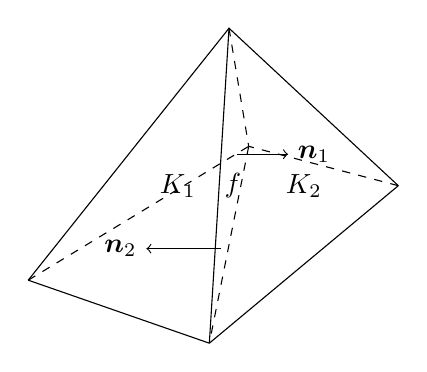
\begin{tikzpicture}
		\draw (0.8,0) -- (3.2,2.0);
		\draw[dashed] (3.2,2.0) -- (1.3,2.5);
		\draw[dashed] (1.3,2.5) -- (0.8,0);
		\draw (0.8,0) -- (-1.5,0.8);
		\draw[dashed] (-1.5,0.8) -- (1.3,2.5);
		\draw (-1.5,0.8) -- (1.05,4) -- (3.2,2.0);
		\draw (1.05,4) -- (0.8,0);
		\draw[dashed] (1.05,4) -- (1.3,2.5); 
		\node (A) at (0.4,2.0) {$K_1$};
		\node (B) at (2.0,2.0) {$K_2$};
		\node (C) at (1.1,2) {$f$};
		\draw[->] (1.15,2.4) -- (1.8,2.4)node[right]{$\boldsymbol{n}_1$};
		\draw[->] (0.95,1.2) -- (0,1.2)node[left]{$\boldsymbol{n}_2$};
	\end{tikzpicture}
	\caption{Two adjacent tetrahedral elements and a common face}
	\label{Fig5.1}
\end{figure}


Now rewrite equation (\ref{eqn1.1}) as a first-order system:
\begin{align}\label{eqn1.3}
	\pb&=\mu^{-1}\nabla\times \Eb \quad \text{in }\Omega,\\\label{eqn1.4}
	\epsilon \Eb+\nabla\times\pb+\Jb&=\tilde{\lb}\qquad\qquad\;\,\,\,\,\text{in }\Omega.
\end{align}
Multiplying both sides of equation (\ref{eqn1.3}) and equation (\ref{eqn1.4}) by test functions $\qb, \vb \in \Hb(\curlb, \Omega)$, respectively, and integrating over $K \in \mathcal{T}_h$, we use formula (\ref{eqnpar}) to obtain
\begin{align}\label{eqn1.5}
	&\int_K\pb\cdot\qb\mathrm{d}\xb=\int_K\Eb\cdot(\nabla\times(\mu^{-1}\qb))\mathrm{d}\xb+\int_{\partial K}(\Eb\times(\mu^{-1}\qb))\cdot\nb_K\mathrm{d}S,\\\label{eqn1.6}
	&\int_K\epsilon\Eb\cdot\vb\mathrm{d}\xb+\int_K\pb\cdot(\nabla\times\vb)\mathrm{d}\xb+\int_{\partial K}(\pb\times\vb)\cdot\nb_K\mathrm{d}S+\int_K\Jb\cdot \vb\mathrm{d}\xb=\int_K\tilde{\lb}\cdot \vb\mathrm{d}\xb.
\end{align}
Here, $\nb_K$ is the outward unit normal vector on $\partial K$. The condition (\ref{eqn1.2}) implies
\begin{equation*}
	\int_K \Jb\cdot\vb\mathrm{d}\xb \leq \int_K\psi^0(\Eb;\vb)\mathrm{d}\xb.
\end{equation*}
So, we derive from equation (\ref{eqn1.6}) that
\begin{equation}\label{eqn1.7}
\int_K\epsilon\Eb\cdot\vb\mathrm{d}\xb+\int_K\pb\cdot(\nabla\times\vb)\mathrm{d}\xb+\int_{\partial K}(\pb\times\vb)\cdot\nb_K\mathrm{d}S+ \int_K\psi^0(\Eb;\vb)\mathrm{d}\xb\geq	\langle \fb ,\vb\rangle.
\end{equation}

Given a positive integer $l$, we introduce the following DG space
\begin{equation*}
    \Vb_h=\{\vb\in\Lb^2(\Omega):\vb|_K\in\boldsymbol{P}^l(K)\ \forall\, K\in\mathcal{T}_h\},%\cap H_0(\text{curl};\Omega).
\end{equation*}
where $\boldsymbol{P}^l(K)=P^l(K)^3$ and $P^l(K)$ is the space of polynomials of a degree less than or equal to $l$ on $K$.
Numerical fluxes $\widehat{\Eb_h}$ and $\widehat{\pb_h}$ are used to approximate the values of $\Eb$ and $\pb$ on $\partial K$, and $\Eb_h$ and $\pb_h$ are used to approximate $\Eb$ and $\pb$ on $K$.  
We derive from (\ref{eqn1.5}) and (\ref{eqn1.7}) that
\begin{align*}	&\int_K\pb_h\cdot\qb_h\mathrm{d}\xb=\int_K\Eb_h\cdot(\nabla\times(\mu^{-1}\qb_h))\mathrm{d}\xb+\int_{\partial K}(\widehat{\Eb_h}\times(\mu^{-1}\qb_h))\cdot\nb_K\mathrm{d}S,\quad  \\
&\int_K\epsilon\Eb_h\cdot\vb_h\mathrm{d}\xb+\int_K\pb_h\cdot(\nabla\times\vb_h)\mathrm{d}\xb+\int_{\partial K}(\widehat{\pb_h}\times\vb_h)\cdot\nb_K\mathrm{d}S+\int_K\psi^0(\Eb_h;\vb_h)\mathrm{d}\xb\geq	\langle \fb ,\vb_h\rangle,
\end{align*}
where $\Eb_h, \pb_h \in \Vb_h$. Summing the integrals over all tetrahedral elements, we obtain
\begin{align}\label{eqn1.8}	\int_\Omega\pb_h\cdot\qb_h\mathrm{d}\xb&=\int_\Omega\Eb_h\cdot\nabla_h\times(\mu^{-1}\qb_h)\mathrm{d}\xb+\sum_{K\in\mathcal{T}_h}\int_{\partial K}(\widehat{\Eb_h}\times(\mu^{-1}\qb_h))\cdot\nb_K\mathrm{d}S \quad\forall \qb_h\in\Vb_h, \\\notag
\int_\Omega\epsilon\Eb_h\cdot\vb_h\mathrm{d}\xb&+\int_\Omega\pb_h\cdot\nabla_h\times\vb_h\mathrm{d}\xb+\sum_{K\in\mathcal{T}_h}\int_{\partial K}(\widehat{\pb_h}\times\vb_h)\cdot\nb_K\mathrm{d}S\\\label{eqn1.9}&+\int_\Omega\psi^0(\Eb_h;\vb_h)\mathrm{d}\xb\ge\langle \fb ,\vb_h\rangle\quad\forall\vb_h\in\Vb_h,
\end{align}
where $\nabla_h \times$ denotes the piecewise curl operator applied to functions over each tetrahedral element $K$, that is, $\nabla_h \times (\vb_h|_K) = \nabla\times (\vb_h|_K)$ $\forall\,K \in\mathcal{T}_h$.

It can be shown that the following equation holds for two vector functions $\vb$ and $\qb$:
\begin{equation}\label{eqn1.11}
\begin{aligned}    \sum_{K\in\mathcal{T}_h}\int_{\partial K}(\vb\times\qb)\cdot\nb_K\mathrm{d}S&=\sum_{f\in\mathcal{F}_h^{\mathcal{I}}}\int_f \llbracket\vb\rrbracket\cdot\{\qb\}\mathrm{d}S-\sum_{f\in\mathcal{F}_h}\int_f\llbracket\qb\rrbracket\cdot\{\vb\}\mathrm{d}S\\
&=\sum_{f\in\mathcal{F}_h}\int_f \llbracket\vb\rrbracket\cdot\{\qb\}\mathrm{d}S-\sum_{f\in\mathcal{F}_h^{\mathcal{I}}}\int_f\llbracket\qb\rrbracket\cdot\{\vb\}\mathrm{d}S.
\end{aligned}
\end{equation}
By utilizing equations (\ref{eqnpar}) and (\ref{eqn1.11}), we can rewrite (\ref{eqn1.8}) and (\ref{eqn1.9}) as follows:
\begin{align}\notag
	\int_\Omega\pb_h\cdot\qb_h\mathrm{d}\xb&=\int_\Omega(\nabla_h\times\Eb_h)\cdot(\mu^{-1}\qb_h)\mathrm{d}\xb+\sum_{f\in\mathcal{F}_h}\int_f  \llbracket\widehat{\Eb_h}-\Eb_h\rrbracket\cdot\{\mu^{-1}\qb_h\}\mathrm{d}S
	\\\label{eqn1.12}
	&\quad{}-\sum_{f\in\mathcal{F}_h^{\mathcal{I}}}\int_f\llbracket\mu^{-1}\qb_h\rrbracket\cdot\{\widehat{\Eb_h}-\Eb_h\}\mathrm{d}S,  
	\\\notag
	\int_\Omega\epsilon\Eb_h\cdot\vb_h\mathrm{d}\xb&+\int_\Omega\pb_h\cdot(\nabla_h\times\vb_h)\mathrm{d}\xb+\sum_{f\in\mathcal{F}_h^{\mathcal{I}}}\int_f \llbracket\widehat{\pb_h}\rrbracket\cdot\{\vb_h\}\mathrm{d}S
	\\\label{eqn1.13}
	&{}-\sum_{f\in\mathcal{F}_h}\int_f\llbracket\vb_h\rrbracket\cdot\{\widehat{\pb_h}\}\mathrm{d}S   
	+\int_\Omega\psi^0(\Eb_h;\vb_h)\mathrm{d}\xb\geq	\langle \fb ,\vb_h\rangle.
\end{align}
We set $\qb_h=\nabla_h\times\vb_h$ in equation (\ref{eqn1.12}) to obtain
\begin{align}
	\notag
	\int_\Omega\pb_h\cdot(\nabla_h\times\vb_h)\mathrm{d}\xb=&\int_\Omega\mu^{-1}(\nabla_h\times\Eb_h)\cdot(\nabla_h\times\vb_h)\mathrm{d}\xb\\\notag
	&+\sum_{f\in\mathcal{F}_h}\int_f \llbracket\widehat{\Eb_h}-\Eb_h\rrbracket\cdot\{\mu^{-1}\nabla_h\times\vb_h\}\mathrm{d}S
	\\\label{eqn1.14}
	&-\sum_{f\in\mathcal{F}_h^{\mathcal{I}}}\int_f\llbracket\mu^{-1}\nabla_h\times\vb_h\rrbracket\cdot\{\widehat{\Eb_h}-\Eb_h\}\mathrm{d}S,  
\end{align}
Substituting equation (\ref{eqn1.14}) into (\ref{eqn1.13}), we obtain the DG scheme
\begin{equation}\label{eqn1.15}	
a_h(\Eb_h,\vb_h)+\int_\Omega\psi^0(\Eb_h;\vb_h)\mathrm{d}\xb\geq\langle \fb ,\vb_h\rangle\quad\forall\,\vb_h\in\Vb_h.
\end{equation}
Here, the bilinear form $a_h(\Eb_h,\vb_h)$ is defined as
\begin{align}\notag
	a_h(\Eb_h,\vb_h)=&\int_\Omega\epsilon\Eb_h\cdot\vb_h\mathrm{d}\xb+\int_\Omega\mu^{-1}(\nabla_h\times\Eb_h)\cdot(\nabla_h\times\vb_h)\mathrm{d}\xb
	\\\notag
	&+\sum_{f\in\mathcal{F}_h}\int_f\llbracket\widehat{\Eb_h}-\Eb_h\rrbracket\cdot\{\mu^{-1}\nabla_h\times\vb_h\}\mathrm{d}S
	\\\notag
	&-\sum_{f\in\mathcal{F}_h^{\mathcal{I}}}\int_f\llbracket\mu^{-1}\nabla_h\times\vb_h\rrbracket\cdot\{\widehat{\Eb_h}-\Eb_h\}\mathrm{d}S 
	\\\label{eqn1.16}
	&+\sum_{f\in\mathcal{F}_h^{\mathcal{I}}}\int_f \llbracket\widehat{\pb_h}\rrbracket\cdot\{\vb_h\}\mathrm{d}S
	-\sum_{f\in\mathcal{F}_h}\int_f\llbracket\vb_h\rrbracket\cdot\{\widehat{\pb_h}\}\mathrm{d}S.   
\end{align}

Define $h_f$ on $f \in \mathcal{F}_h$ as 
\begin{align*}
	h_f=\begin{cases}
		\min \{h_K,h_{K'}\} \quad f\in\mathcal{F}_h^{\mathcal{I}}, \quad f =\partial K \cap \partial K',\\
		h_K \quad \quad \qquad \quad  \text{ } \textbf{ }f \in \mathcal{F}_h^{\mathcal{B}},\quad f=\partial K \cap \partial \Omega.
	\end{cases}
\end{align*}
Let $\eta>0$ be a constant and define $\alpha$ on each $f \in \mathcal{F}_h$ by the formula
\[ \alpha|_f=\eta h_f^{-1}.\]
We may choose a different constant $\eta$ for each $f\in \mathcal{F}_h$ and the following discussions still go through. Choose the numerical fluxes as
\begin{equation*}
\begin{cases}
\widehat{\Eb_h}=\{\Eb_h\}\qquad\qquad\qquad\qquad\,\,\,\,\text{on } \mathcal{F}_h^{\mathcal{I}} , \\
{\nb\times\widehat{\Eb_h}}=\zerob \qquad\qquad\qquad\qquad\,\,\,\,\text{on } \mathcal{F}_h^{\mathcal{B}} , \\
\widehat{\pb_h}=\{\mu^{-1}\nabla_h\times\Eb_h\}-\alpha\llbracket\Eb_h\rrbracket \quad \text{on } \mathcal{F}_h.
\end{cases}
\end{equation*}
Using these choices in (\ref{eqn1.16}), we obtain the bilinear form for the IPDG scheme: 
\begin{align}\notag
	a_h(\Eb_h,\vb_h)&=\int_\Omega\epsilon \Eb_h\cdot \vb_h \mathrm{d}\xb+\int_\Omega\mu^{-1}(\nabla_h\times\Eb_h)\cdot(\nabla_h\times\vb_h)\mathrm{d}\xb
	\\\notag
	&\quad{}-\sum_{f\in\mathcal{F}_h}\int_f\llbracket\Eb_h\rrbracket\cdot\{\mu^{-1}\nabla_h\times\vb_h\}\mathrm{d}S-\sum_{f\in\mathcal{F}_h}\int_f\llbracket\vb_h\rrbracket\cdot\{\mu^{-1}\nabla_h\times\Eb_h\}\mathrm{d}S
	\\\label{eqn1.17}
	&\quad{}+\sum_{f\in\mathcal{F}_h}\int_f \alpha\llbracket\Eb_h\rrbracket\cdot\llbracket\vb_h\rrbracket\mathrm{d}S.
\end{align}
With the discrete bilinear form $a_h(\cdot, \cdot)$ defined by (\ref{eqn1.17}), the IPDG scheme to solve the $\Hcurlb$-elliptic hemivariational inequality is to find $\Eb_h \in \Vb_h$ such that
\begin{equation}\label{eqn1.18}
a_h(\Eb_h,\vb_h)+\int_\Omega\psi^0(\Eb_h;\vb_h)\mathrm{d}\xb \geq\langle \fb,\vb_h\rangle\quad \forall \vb_h\in\Vb_h.
\end{equation}



\section{Error analysis}
In this section, we study some properties of the IPDG scheme and provide a priori error estimates. On several occasions, we will apply the modified Cauchy-Schwarz inequality with an arbitrarily small parameter $\varepsilon>0$:
\begin{equation}
a\,b\le \varepsilon\,a^2+\frac{1}{4\varepsilon}\,b^2\quad\forall\,a,b\in\mathbb{R}.
\label{mCS}
\end{equation}

\subsection{Properties of the IPDG scheme}

This section is devoted to the consistency, stability, boundedness of the IPDG scheme, and uniform boundedness of its numerical solution.

\begin{theorem}[Consistency]
The IPDG scheme \eqref{eqn1.18} is consistent, i.e., for the solution $\Eb\in\Vb \cap\Hb^2(\Omega)$ of the problem \eqref{eqn1.1}--\eqref{eqn1.2}, 
\begin{equation}
a_h(\Eb,\vb_h)+\int_\Omega\psi^0(\Eb;\vb_h)\mathrm{d}\xb\ge\langle\fb,\vb_h\rangle\quad\forall\,\vb_h\in\Vb_h.
\label{eq:cons}
\end{equation}
\end{theorem}
\begin{proof}
The discrete bilinear form (\ref{eqn1.17}) is defined with $\Eb_h$ replaced by $\Eb$.  Applying equation (\ref{eqn1.11}), we notice that the fourth term of $a_h(\Eb,\vb_h)$ is
\begin{equation}
  \begin{aligned}
    -\sum_{f\in\mathcal{F}_h}\int_f\llbracket\vb_h\rrbracket\cdot\{\mu^{-1}\nabla\times\Eb\}\mathrm{d}S=&-\sum_{K\in\mathcal{T}_h}\int_{\partial K}\mu^{-1}(\vb_h\times\nabla\times\Eb)\cdot \nb_K\mathrm{d}S
    \\
     &-\sum_{f\in\mathcal{F}_h^{\mathcal{I}}}\int_f\llbracket\mu^{-1}\nabla\times\Eb\rrbracket\cdot\{\vb_h\}\mathrm{d}S.
  \end{aligned}
\end{equation} 
Moreover, $\llbracket \Eb \rrbracket = \zerob$ on $\mathcal{F}_h$ and $\llbracket \nabla\times \Eb \rrbracket = \zerob$ on $\mathcal{F}_h^{\mathcal{I}}$. Therefore, 
\begin{align*}
a_h(\Eb,\vb_h) & =\int_\Omega\epsilon \Eb\cdot\vb_h\mathrm{d}\xb+\int_\Omega\mu^{-1}(\nabla\times\Eb)\cdot(\nabla_h\times\vb_h)\mathrm{d}\xb\\
&\quad{} -\sum_{K\in\mathcal{T}_h}\int_{\partial K}\mu^{-1}(\vb_h\times\nabla\times\Eb)\cdot \nb_K\mathrm{d}S.
\end{align*}
Applying the integration by parts formula (\ref{eqnpar}) on the integration region $K\in\mathcal{T}_h$, we have
\begin{align*}
\int_K\mu^{-1}(\nabla\times\Eb)\cdot(\nabla\times\vb_h)\mathrm{d}\xb
& =\int_K\nabla\times(\mu^{-1}\nabla\times\Eb)\cdot\vb_h\mathrm{d}\xb\\
&\quad{} -\int_{\partial K}\mu^{-1}((\nabla\times\Eb)\times\vb_h)\cdot\nb_K\mathrm{d}S.
\end{align*}
Thus,
\begin{equation*}
	a_h(\Eb,\vb_h)=\int_\Omega\epsilon \Eb\cdot\vb_h\mathrm{d}\xb+\int_\Omega\nabla\times(\mu^{-1}\nabla\times\Eb)\cdot\vb_h\mathrm{d}\xb.
\end{equation*}
Multiplying both sides of equation (\ref{eqn1.1}) by a function $\vb_h \in \Vb_h$ and integrating over $\Omega$, we obtain
\[
\int_\Omega\epsilon\Eb\cdot\vb_h\mathrm{d}\xb+\int_\Omega\nabla\times(\mu^{-1}\nabla\times\Eb)\cdot\vb_h\mathrm{d}\xb+\int_\Omega \Jb \cdot \vb_h\mathrm{d}\xb=\int_\Omega\tilde{\lb}\cdot \vb_h\mathrm{d}\xb.
\]
Since $\Jb \in \partial \psi(\Eb)$ and by the definition of the functional $\fb \in \Vb^*$, \eqref{eq:cons} follows.
\end{proof}

Let
\[\Vb(h) = \Hb_0(\curlb; \Omega) + \Vb_h\]
with the semi-norm and norm defined by
\begin{equation*}
{|\vb|_h^2=\sum_{K\in\mathcal{T}_h}\| \nabla\times\vb\|_{0,K}^2+\sum_{f\in\mathcal{F}_h}\| \alpha^{1/2}\llbracket\vb\rrbracket\|_{0,f}^2,\quad \|\vb\|_h^2=\|\vb\|_{0,\Omega}^2+|\vb|_h^2.}
\end{equation*}
The bilinear form $a_h(\cdot,\cdot)$ is initially defined on $\Vb_h\times\Vb_h$. To extend it to $\Vb(h)\times\Vb(h)$, we introduce an auxiliary bilinear form as follows\textsuperscript{\cite{grote2007interior, perugia2002hp}}
\begin{align}\label{eqn2.2}
\widetilde{a}_h(\Eb,\vb)&=\int_\Omega\epsilon \Eb\cdot \vb \mathrm{d}\xb+\widetilde{b}_h(\Eb,\vb),
\end{align}
where
\begin{align*}
\widetilde{b}_h(\Eb,\vb)=&\sum_{K\in\mathcal{T}_h}\int_K\mu^{-1}(\nabla\times\Eb)\cdot(\nabla\times\vb)\mathrm{d}\xb
-\sum_{f\in\mathcal{F}_h}\int_f\llbracket\Eb\rrbracket\cdot\{\mu^{-1}\Pib_h(\nabla\times\vb)\}\mathrm{d}S
	\\
&-\sum_{f\in\mathcal{F}_h}\int_f\llbracket\vb\rrbracket\cdot\{\mu^{-1}\Pib_h(\nabla\times\Eb)\}\mathrm{d}S+\sum_{f\in\mathcal{F}_h}\int_f\alpha\llbracket\Eb\rrbracket\cdot\llbracket\vb\rrbracket\mathrm{d}S.
\end{align*} 
Here, $\Pib_h$ is an $L^2$-projection from $\Vb(h)$ to $\Vb_h$. Note that $\widetilde{a}_h(\cdot,\cdot)$ coincides with $a_h(\cdot,\cdot)$ on $\Vb_h\times\Vb_h$. 

\begin{lemma}[Boundedness]\label{lemma:boundeness}
There is a constant $C_b>0$ such that
\begin{equation}
\tilde{a}_h(\Eb,\vb)\leq C_b\|\Eb\|_h \|\vb\|_h\quad \forall\,\Eb,\vb\in\Vb(h). 
\label{ah:bd}
\end{equation}
\end{lemma}
\begin{proof}
Using H\"{o}lder's inequality, we can get
\begin{equation*}
\begin{aligned}   			   		
\int_K\mu^{-1}(\nabla\times\Eb)\cdot(\nabla\times\vb)\mathrm{d}\xb 
&\leq \mu_0^{-1}\int_K|\nabla\times\Eb|\cdot|\nabla\times\vb|\mathrm{d}\xb\\
&\leq \mu_0^{-1}\|\nabla_h\times \Eb \|_{0,K}\|\nabla_h\times \vb \|_{0,K}.
\end{aligned}
\end{equation*}
Similarly,
\begin{align*}
\int_f \alpha\llbracket \Eb \rrbracket \cdot \llbracket \vb \rrbracket \mathrm{d}S 
&\leq  \| \alpha^{1/2}\llbracket\Eb\rrbracket\|_{0,f}\| \alpha^{1/2}\llbracket\vb\rrbracket\|_{0,f},\\
\int_\Omega\epsilon \Eb\cdot \vb \mathrm{d}\xb & \leq\epsilon_1\|\Eb\|_{0,\Omega}\|\vb\|_{0,\Omega}.
\end{align*}
Now let us bound the third term of the bilinear form $\tilde{a}_h(\cdot,\cdot) $ which is a modification of the proof of \cite[Lemma 4]{grote2007interior}.
\begin{equation*}
\begin{aligned}
&\sum_{f\in\mathcal{F}_h}\int_f\llbracket\Eb\rrbracket\cdot\{\mu^{-1}\Pib_h(\nabla_h\times\vb)\}\mathrm{d}S
\\
\leq &\mu_0^{-1}\sum_{f\in\mathcal{F}_h}\int_f\left|\alpha^{1/2}\llbracket\Eb\rrbracket\right|\cdot\left|\alpha^{-1/2}\{\Pib_h(\nabla_h\times\vb)\}\right|\mathrm{d}S   \\
\leq &\mu_0^{-1}\sum_{f\in\mathcal{F}_h} \|\alpha^{1/2}\llbracket\Eb\rrbracket\|_{0,f} \cdot \|\alpha^{-1/2}\{\Pib_h(\nabla_h\times\vb)\}\|_{0,f} 
\\
\leq &\mu_0^{-1}\left(\sum_{f\in\mathcal{F}_h} \int_f\alpha\left|\llbracket\Eb\rrbracket\right|^2 \mathrm{d}S\right)^{1/2} \cdot
\left(\sum_{f\in\mathcal{F}_h} \int_f\alpha^{-1} \left| \{\Pib_h(\nabla_h\times\vb)\} \right|^2 \mathrm{d}S\right)^{1/2}
\\
= & 
\mu_0^{-1}\eta^{-1/2}\left(\sum_{f\in\mathcal{F}_h} \|\alpha^{1/2}\llbracket\Eb\rrbracket\|^2_{0,f}\right)^{1/2} \cdot\left(\sum_{f\in\mathcal{F}_h} \int_f  h_f\left| \{\Pib_h(\nabla_h\times\vb)\} \right|^2 \mathrm{d}S\right)^{1/2}.
\end{aligned}
\end{equation*}
Using the definition of $h_f$, we can get
\begin{equation*}
\begin{aligned}
\sum_{f\in\mathcal{F}_h} \int_f  h_f \left| \{\Pib_h(\nabla_h\times\vb)\} \right|^2 \mathrm{d}S&\leq \frac{1}{2}\sum_{K\in\mathcal{T}_h}\int_{\partial K}h_K  |\Pib_h(\nabla\times \vb)|^2 \mathrm{d}S
\\
& \leq \frac{1}{2}\sum_{K\in\mathcal{T}_h}h_K\| \Pib_h(\nabla\times \vb)\|^2_{0,\partial K}. 
\end{aligned}
\end{equation*}
Recalling the trace theorem\textsuperscript{\cite[Chapter 5.5, Theorem 1]{evans2022partial}} and inverse inequality\textsuperscript{\cite[Lemma (4.5.3)]{brenner2008mathematical}} 
\[
\| \wb \|^2_{0,\partial K} \leq C_{tr}^2 \|\wb\|^2_{W^{1,2}(K)} \leq C_{tr}^2C_{inv}^2 h^{-1}_K \| \wb\|_{0,K}^2
\quad \forall\, \wb\in\boldsymbol{P}^l(K),\ \forall\, K\in\mathcal{T}_h,
\]
where the positive constants $C_{tr}$ and $C_{inv}$ depend only on the regularity of the mesh and the polynomial degree $l$ of the finite element space. Henceforth, we use $\tilde{C}$ to replace $C_{tr}C_{inv}$. From the $L^2$-projection property,
\[
\| \Pib_h \wb \|_{0,K} \leq \|\wb \|_{0,K} \quad \forall\, \wb \in \Lb^2(K).
\]
Then, combining the above result, we can obtain 
\begin{equation*}
\frac{1}{2}\sum_{K\in\mathcal{T}_h}h_K\|  \Pib_h(\nabla\times \vb)\|^2_{0,\partial K}\leq \frac{1}{2}\tilde{C}^2\sum_{K\in\mathcal{T}_h} \|\nabla\times \vb\|^2_{0,K}.
\end{equation*}
Finally, we obtain the bound
\begin{equation}
\begin{aligned}
\sum_{f\in\mathcal{F}_h}\int_f\llbracket\Eb\rrbracket\cdot\{\mu^{-1}\Pib_h(\nabla_h\times\vb)\}\mathrm{d}S 
\leq &
\mu_0^{-1}(2\eta)^{-1/2}\tilde{C} \left(\sum_{f\in\mathcal{F}_h} \|\alpha^{1/2}\llbracket\Eb\rrbracket\|^2_{0,f}\right)^{1/2} 
\\
& 
\cdot \left(\sum_{K\in\mathcal{T}_h} \|\nabla\times \vb\|^2_{0,K} \right)^{1/2}
\end{aligned} 
\end{equation}
Similarly, we can bound the fourth term of the bilinear form as 
\begin{equation}
\begin{aligned}
\sum_{f\in\mathcal{F}_h}\int_f\llbracket\vb\rrbracket\cdot\{\mu^{-1}\nabla_h\times\Eb\}\mathrm{d}S
\leq &
\mu_0^{-1}(2\eta)^{-1/2}\tilde{C} \left(\sum_{f\in\mathcal{F}_h} \|\alpha^{1/2}\llbracket\vb\rrbracket\|^2_{0,f}\right)^{1/2} 
\\
& 
\cdot \left(\sum_{K\in\mathcal{T}_h} \| \nabla\times \Eb\|^2_{0,K} \right)^{1/2}.
\end{aligned}
\end{equation}
Combining these results, we get \eqref{ah:bd}.
\end{proof}

\begin{lemma}[Stability]\label{lemma:stability}
Assume $\eta > \max\{1,\mu_1^2\}\,\tilde{C}^2/(2\,\mu_0^2)$.  There is a constant $C_s>0$ such that
\begin{equation}
\tilde{a}_h(\Eb,\Eb)\geq C_s \|\Eb\|_h^2, \quad \forall \Eb\in\Vb(h).
\label{eqn2.5}
\end{equation}
\end{lemma}
\begin{proof}
\[
\int_\Omega\epsilon \Eb\cdot \Eb \mathrm{d}\xb \geq \epsilon_0\|  \Eb\|_{0,\Omega}^2 ,
\]
\[	\sum_{K\in\mathcal{T}_h}\int_K\mu^{-1}(\nabla\times\Eb)\cdot(\nabla\times\Eb)\mathrm{d}\xb \geq\mu_1^{-1}\sum_{K\in\mathcal{T}_h} \|\nabla_h\times \Eb \|_{0,K}^2,
\]
\[
\sum_{f\in\mathcal{F}_h}\int_f \alpha\llbracket\Eb\rrbracket\cdot\llbracket\Eb\rrbracket\mathrm{d}S=\sum_{f\in\mathcal{F}_h}\| \alpha^{1/2}\llbracket\Eb\rrbracket\|_{0,f}^2.
\]
Similar to the proof of Lemma \ref{lemma:boundeness}, we have
\begin{align*}
&-2\sum_{f\in\mathcal{F}_h}\int_f\llbracket\Eb\rrbracket\cdot\{\mu^{-1}\Pib_h(\nabla\times\Eb)\}\mathrm{d}S
\\
\geq&-2\mu_0^{-1}(2\eta)^{-1/2}\tilde{C}\left(\sum_{f\in\mathcal{F}_h}\| \alpha^{1/2}\llbracket\Eb\rrbracket\|_{0,f}^2\right)^{1/2} \cdot \left( \sum_{K\in\mathcal{T}_h}\|\nabla\times \Eb\|_{0,K}^2 \right)^{1/2}
\\
\geq&-\mu_0^{-1}(2\eta)^{-1/2}\tilde{C}\left(\sum_{f\in\mathcal{F}_h}\| \alpha^{1/2}\llbracket\Eb\rrbracket\|_{0,f}^2+\sum_{K\in\mathcal{T}_h}\|\nabla\times \Eb\|_{0,K}^2 \right).
\end{align*}
Therefore, when $\eta > \max\{1,\mu_1^2\}\,\tilde{C}^2/(2\,\mu_0^2)$, $\tilde{a}_h(\Eb,\Eb)$ is bounded from below by
\begin{equation}\label{lower bound of tiled{a}}
\begin{aligned}
&\epsilon_0\|  \Eb\|_{0,\Omega}^2 + \left(1-\mu_0^{-1}(2\eta)^{-1/2}\tilde{C}\right)\sum_{f\in\mathcal{F}_h}\| \alpha^{1/2}\llbracket\Eb\rrbracket\|_{0,f}^2 \\
&+\left(\mu_1^{-1}-\mu_0^{-1}(2\eta)^{-1/2}\tilde{C}\right)\sum_{K\in\mathcal{T}_h}\|\nabla\times \Eb\|_{0,K}^2.
\end{aligned}
\end{equation}
Denote $C_0 = 1-\mu_0^{-1}(2\eta)^{-1/2}\tilde{C}$, $C_1 = \mu_1^{-1}-\mu_0^{-1}(2\eta)^{-1/2}\tilde{C}$.  Then,
\[ \tilde{a}_h(\Eb,\Eb) \geq C_s\left(\sum_{f\in\mathcal{F}_h}\| \alpha^{1/2}\llbracket\Eb\rrbracket\|_{0,f}^2+\sum_{K\in\mathcal{T}_h}\|\nabla\times \Eb\|_{0,K}^2+\| \Eb\|_{0,\Omega}^2 \right) \] holds, where $C_s = \min\{\epsilon_0, C_0, C_1\}$.
\end{proof}

The next result explores the uniform boundedness of the numerical solution defined by the IPDG scheme for solving the $\Hcurlb$-elliptic hemivariational inequality.

\begin{lemma} 
Assume \eqref{eqn1.other}, $m<\epsilon_0$ and $\eta > \max\{1,\mu_1^2\}\,\tilde{C}^2/(2\,\mu_0^2)$. If $\Eb_h\in \Vb_h$ is a solution of the problem \eqref{eqn1.18}, then $\|\Eb_h\|_h$ is uniformly bounded with respect to the mesh size $h$. 
\end{lemma}
\begin{proof}
By setting $\vb_h=-\Eb_h$ in (\ref{eqn1.18}), we obtain
\begin{equation}\label{eqn2.6}
	a_h(\Eb_h,\Eb_h) \leq \int_\Omega\psi^0(\Eb_h;-\Eb_h) \mathrm{d}\xb +\langle \fb,\Eb_h \rangle.
\end{equation}
From assumption (\ref{eqn1.other})\,(d), we have
\begin{equation*}
	\psi^0(\Eb_h;\zerob-\Eb_h) + \psi^0(\zerob;\Eb_h-\zerob) \leq m|\Eb_h|^2,
\end{equation*}
Using (\ref{eqn1.other2}) to get
\[  -\psi^0(\zerob;\Eb_h)\leq c_0|\Eb_h|; \]
hence,
\begin{equation*}
\int_\Omega\psi^0(\Eb_h;-\Eb_h) \mathrm{d}\xb \leq m\|\Eb_h\|_{0,\Omega}^2 + \int_\Omega c_0|\Eb_h| \mathrm{d}\xb.
\end{equation*}
Moreover,
\[ \langle \fb,\Eb_h\rangle\leq\| \fb \|_{\Vb^*}\| \Eb_h\|_{\curlb,\Omega}\leq \| \fb \|_{\Vb^*} \|\Eb_h\|_h.\]
By the Cauchy-Schwarz inequality, 
\[
\int_\Omega c_0 |\Eb_h|\mathrm{d}\xb \leq c_0 |\Omega|^{1/2}\| \Eb_h \|_{0,\Omega},
\]
where $|\Omega|$ means the Lebesgue measurement of the bounded domain $\Omega$. Combine these inequalities with the lower bound (\ref{lower bound of tiled{a}}) of $\tilde{a}(\Eb_h, \Eb_h)$ to get
\begin{align*}
&(\epsilon_0-m)\|  \Eb\|_{0,\Omega}^2 + C_0\sum_{f\in\mathcal{F}_h}\| \alpha^{1/2}\llbracket\Eb\rrbracket\|_{0,f}^2 + C_1 \sum_{K\in\mathcal{T}_h}\|\nabla\times \Eb\|_{0,K}^2	\\
&\leq \left(c_0|\Omega|^{-1/2}+\|\fb\|_{\Vb^*}  \right)\|\Eb_h\|_h .
\end{align*}
Since $\epsilon_0-m>0$ and $\eta > \max\{1,\mu_1^2\}\,\tilde{C}^2/(2\,\mu_0^2)$, then
\begin{equation}
\|\Eb_h\|_h \leq \frac{c_0|\Omega|^{-1/2}+\|\fb\|_{\Vb^*}}{\min\{\epsilon_0-m, C_0, C_1\}}.
\end{equation}
Therefore, $\|\Eb_h\|_h$ is bounded by a constant independent of $h$.
\end{proof}

Since $\epsilon_0 = k^{-1} \tilde{\epsilon}_0$, the condition $m<\epsilon_0$ can always be satisfied as long as the time step-size $k$ is sufficiently small.

\subsection{Existence and uniqueness}
In this subsection, we present the existence and uniqueness of the solution of (\ref{eqn1.18}) following the idea presented in \cite{han2020minimization, han2022numerical}. Define an energy functional 
\begin{equation}
\mathcal{E}(\vb_h) = \frac{1}{2}a_h(\vb_h, \vb_h)+\int_\Omega \psi(\vb_h) \mathrm{d}\xb - \langle \fb, \vb_h \rangle, \quad \vb_h \in \Vb_h.
\end{equation}
We consider the minimization problem
\begin{equation}\label{minimization problem}
\Eb_h \in \Vb_h, \quad \mathcal{E}(\Eb_h) = \inf\{\mathcal{E}(\vb_h) \mid \vb_h\in\Vb_h\}.
\end{equation}

\begin{lemma}
Assume \eqref{eqn1.other}, $m<\epsilon_0$ and $\eta > \max\{1,\mu_1^2\}\,\tilde{C}^2/(2\,\mu_0^2)$. Then the functional $\mathcal{E}(\cdot)$ is locally Lipschitz continuous, strongly convex and coercive on $\Vb_h$.
\end{lemma}
\begin{proof}
The local Lipschitz continuity of $\mathcal{E}(\cdot)$ is obvious.
Let us prove the strong convexity.
For this purpose, define a linear operator $A_h \colon \Vb_h \to \Vb_h^*$ by
\begin{equation}
\label{eq:4.3}
\langle A_h \ub_h, \vb_h\rangle \;=\; a_h(\ub_h,\vb_h)
\quad
\forall\,\ub_h,\vb_h \in \Vb_h.
\end{equation}
Applying Lemma~\ref{lemma:boundeness}, we obtain 
\begin{equation*}
\|A_h\ub_h\|_{\Vb_h^*} = \sup_{\|\vb_h\|_h \ne 0} \frac{|\langle A_h\ub_h, \vb_h\rangle|}{\|\vb_h\|_h} = \sup_{\|\vb_h\|_h \ne 0} \frac{|a_h(\ub_h, \vb_h)|}{\|\vb_h\|_h} \leq C_b \|\ub_h\|_h \quad \forall \ub_h \in \Vb_h.
\end{equation*}
By Lemma~\ref{lemma:stability}, 
\begin{equation*}
\begin{aligned}
\langle A_h\ub_h - A_h\vb_h, \ub_h - \vb_h \rangle = a_h(\ub_h - \vb_h, \ub_h - \vb_h) \geq C_s \|\ub_h-\vb_h\|_h^2 \quad \forall  \ub_h, \vb_h \in \Vb_h.
\end{aligned}
\end{equation*}
So $A_h \in \mathcal{L}(\Vb_h, \Vb_h^*)$ and it is strongly monotone. Define a functional $\Psi : \Lb^2(\Omega) \to \mathbb{R}$ by
\[
\Psi(\vb)
\;=\;
\int_\Omega \psi(\vb)\,\mathrm{d}\xb
\quad
\forall\,\vb \in \Lb^2(\Omega).
\]
Then, by \cite[Theorem~3.47]{migorski2013nonlinear}, under assumption (\ref{eqn1.other}), $\Psi$ is well defined, locally Lipschitz continuous on $\Lb^2(\Omega)$, and
\begin{equation}
\label{eq:4.4}
\partial \Psi(\vb)
\;\subset\;
\int_\Omega \partial \psi\bigl(\vb)\,\mathrm{d}\xb
\end{equation}
in the sense that for any $\xib \in \partial \Psi(\vb)$, there exists a function $\zetab \in \Lb^2(\Omega)$ such that $\zetab(\xb) \in \partial \psi\bigl(\xb,\vb(\xb)\bigr)$ for a.e.\ $\xb \in \Omega$ and
\[
\langle \xib,\,\wb\rangle_{\Lb^2(\Omega)\times \Lb^2(\Omega)}
\;=\;
\int_\Omega \zetab(\xb) \cdot \wb(\xb)\,\mathrm{d}\xb
\quad
\forall\,\wb \in \Lb^2(\Omega).
\]
For $\vb_h \in \Vb_h$ and $\etab \in \partial \mathcal{E}(\vb_h)$, by (\ref{subaddition of Clarke}) we can write
\begin{equation}
\label{eqn eta}
\etab = A_h \vb_h + \xib - \fb,
\quad
\xib \in \partial \Psi(\vb_h).
\end{equation}
Thus, for $i=1,2$, with $\vb_{h,i} \in \Vb_h$ and $\etab_i \in \partial \mathcal{E}(\vb_{h,i})$, by \eqref{eq:4.4} we have $\zetab_i \in \Lb^2(\Omega)$ such that $\zetab_i(x) \in \partial \psi\bigl(\xb,\vb_{h,i}(x)\bigr)$ for a.e.\ $\xb \in \Omega$ and
\[
\langle \etab_i, \wb\rangle
\;=\;
\langle A_h \vb_{h,i}, \wb\rangle
\;+\;
\int_\Omega \zetab_i(\xb)\cdot \wb(\xb)\,\mathrm{d}\xb
\;-\;
\langle \fb, \wb\rangle
\quad
\forall\,\wb \in \Lb^2(\Omega).
\]
Thus, from (\ref{property of psi 5}) and Lemma~\ref{lemma:stability},
\begin{equation*}
\begin{aligned}
\langle \etab_1 - \etab_2,\; \vb_{h,1} - \vb_{h,2}\rangle = &\langle A_h \vb_{h,1} - A_h\vb_{h,2}, \vb_{h,1} - \vb_{h,2}\rangle+\int_\Omega \bigl(\zetab_1 - \zetab_2\bigr)\cdot (\vb_1 - \vb_2)\,\mathrm{d}\xb
\\
\geq 
&(\epsilon_0-m)\|  \vb_{h,1} - \vb_{h,2}\|_{0,\Omega}^2 + C_0\sum_{f\in\mathcal{F}_h}\| \alpha^{1/2}\llbracket\vb_{h,1} - \vb_{h,2}\rrbracket\|_{0,f}^2 \\
&+C_1\sum_{K\in\mathcal{T}_h}\|\nabla\times (\vb_{h,1} - \vb_{h,2})\|_{0,K}^2
\\
\geq& \min\{\epsilon_0-m, C_0, C_1\} \| \vb_{h,1} - \vb_{h,2}\|_h.
\end{aligned}
\end{equation*}
Thus, by Lemma~\ref{lem:2.2}, $\mathcal{E}(\cdot)$ is strongly convex.
Moreover, by Proposition~\ref{prop:2.3}, $\mathcal{E}(\cdot)$ is coercive on~$\Vb_h$.
\end{proof}

\begin{proposition}
Under the assumptions \eqref{eqn1.other}, $m<\epsilon_0$ and $\eta > \max\{1,\mu_1^2\}\,\tilde{C}^2/(2\,\mu_0^2)$, the minimization problem \eqref{minimization problem} has a unique solution $\Eb_h \in \Vb_h$
\end{proposition}
\begin{proof}
Since $\mathcal{E}(\cdot)$ is continuous, strictly convex and coercive on $\Vb_h$, from \cite[\S3.3.2]{han2009theoretical} the minimization problem (\ref{minimization problem}) has
a unique solution.
\end{proof}
\begin{theorem}
Assume \eqref{eqn1.other}, $m<\epsilon_0$ and $\eta > \max\{1,\mu_1^2\}\,\tilde{C}^2/(2\,\mu_0^2)$. Then for any $\fb\in \Vb^*$, the problem \eqref{eqn1.18} has a unique solution $\Eb_h\in\Vb_h$, which is also the unique solution of the minimization problem \eqref{minimization problem}.
\end{theorem}
\begin{proof}
For the solution $\Eb_h\in\Vb_h$ of the minimization problem (\ref{minimization problem}), we apply (\ref{eqn eta}) to get
\[
\langle A_h\Eb_h, \vb_h \rangle + \int_\Omega \zetab(\xb)\cdot \vb_h(\xb) \mathrm{d}\xb - \langle \fb, \vb_h \rangle \geq 0,
\]
where $\zetab \in L^2(\Omega)$ such that $\zetab(\xb) \in \partial \psi\bigl(\xb,\vb_h(\xb)\bigr)$ for a.e.\ $\xb \in \Omega$. Using the property of the Clarke subdifferential (\ref{eqnclarke1}) we have
\[
\psi^0(\Eb_h(\xb); \vb_h(\xb)) \geq \zetab(\xb)\cdot \vb_h(\xb_h) \quad \text{a.e. } \xb \in \Omega.
\]
Combining the above two inequalities, we can see that $\Eb_h$ is a solution of the problem (\ref{eqn1.18}). 

Now, let's prove uniqueness of the solution. Assume, $\Eb_h, \tilde{\Eb}_h\in\Vb_h$ are two solutions of the problem (\ref{eqn1.18}). Then we have 
\begin{equation}\label{finite element problem 2}
a_h(\tilde{\Eb}_h,\vb_h)+\int_\Omega\psi^0(\tilde{\Eb}_h;\vb_h)\mathrm{d}\xb \geq\langle \fb,\vb_h\rangle\quad \forall \vb_h\in\Vb_h.
\end{equation}
Take $\vb_h = \tilde{\Eb}_h-\Eb_h$ in (\ref{eqn1.18}) and $\vb_h = \Eb_h-\tilde{\Eb}_h$ in (\ref{finite element problem 2}). Add the two resulting inequalities, combining it with Lemma \ref{lemma:stability} to get 
\begin{equation*}
\begin{aligned}
&\epsilon_0\|  \tilde{\Eb}_h - \Eb_h\|_{0,\Omega}^2 + C_0\sum_{f\in\mathcal{F}_h}\| \alpha^{1/2}\llbracket\tilde{\Eb}_h - \Eb_h\rrbracket\|_{0,f}^2 +C_1\sum_{K\in\mathcal{T}_h}\|\nabla\times (\tilde{\Eb}_h - \Eb_h)\|_{0,K}^2 
\\ 
& \leq a_h(\tilde{\Eb}_h-\Eb_h,\tilde{\Eb}_h-\Eb_h) \leq \int_{\Omega} \left(\psi^0(\Eb_h;\tilde{\Eb}_h - \Eb_h) + \psi^0(\tilde{\Eb}_h; \Eb_h-\tilde{\Eb}_h) \right) \mathrm{d}\xb 
\\
& \leq m \| \tilde{\Eb}_h - \Eb_h \|_{0,\Omega}^2.
\end{aligned}
\end{equation*}
By the smallness condition $m<\epsilon_0$, we deduce that $\tilde{\Eb}_h = \Eb_h$.
\end{proof}


\subsection{A priori error estimate}

The following lemma provides some error bounds for the second type of N\'{e}d\'{e}lec interpolation $\Pib_N$\textsuperscript{\cite{monk2003finite,nedelec1980mixed,nedelec1986new}}.

\begin{lemma}\label{lemma5.4} 
Assume $\{\mathcal{T}_h\}$ is a shape-regular family of tetrahedral or hexahedral mesh partitions of the domain $\overline{\Omega}$, and assume $\Eb \in \Hb_0(\curlb; \Omega) \cap \Hb^s(\Omega)$ with $ \nabla\times \Eb \in \Hb^s(\Omega)$, where $s > 1/2$. Then the following error estimates hold:
\begin{align}
\|\Eb - \Pib_N \Eb\|_{\curlb,\Omega} & \leq C_N h^{\min\{s, l\}} (\|\Eb\|_{s, \Omega} + \|\nabla\times \Eb\|_{s, \Omega}),
\label{eqn:lemma4-1} \\
\|\Eb - \Pib_N \Eb\|_{h} & \leq C_N h^{\min\{s, l\}} (\|\Eb\|_{s, \Omega} + \|\nabla\times \Eb\|_{s, \Omega}),
\label{energy norm estimate}
\end{align}
where $C_N > 0$ is a constant depending on the mesh regularity and the polynomial degree $l$ but independent of $h$, and for \eqref{energy norm estimate}, $C_N$ also depends on the upper and lower bounds of the coefficients $\mu$ and $\epsilon$.
 
Moreover, if $\Eb \in \Hb_0(\curlb; \Omega) \cap \Hb^{s+1}(\Omega)$ for some number $s > 0$, then
\begin{equation}
 \|\Eb - \Pib_N \Eb\|_{0, \Omega} \leq C_N h^{\min\{s, l\}+1} \|\Eb\|_{s+1, \Omega}. 
 \label{eqn:lemma4-3}
 \end{equation} 
\end{lemma}
 
A proof of (\ref{eqn:lemma4-1}) is found in \cite{monk2003finite}, and (\ref{eqn:lemma4-3}) is given as \cite[Lemma 4.1]{houston2005interior}.  The error bound \eqref{energy norm estimate} follows from \eqref{eqn:lemma4-1} since the electric field intensity and magnetic field intensity $\epsilon$ and $\mu$ are bounded and for $\Eb \in \Hb_0(\curlb;\Omega)$, the jump $\llbracket\Eb - \Pib_N \Eb\rrbracket$ vanishes.

For $\vb\in\Vb(h)$, we define
\begin{equation}\label{eqn2.9}
r_h(\Eb;\vb)=\sum_{f\in\mathcal{F}_h}\int_f\llbracket\vb\rrbracket \cdot \left\{\mu^{-1}\nabla\times\Eb-\mu^{-1}\Pib_h(\nabla\times\Eb)\right\}\mathrm{d}S.
\end{equation}
For $r_h(\Eb; \vb)$ to be well-defined, the condition $\nabla\times \Eb \in \Hb^s(\Omega)$, where $s > 1/2$, is assumed. Under this condition, we have the following result\textsuperscript{\cite{grote2007interior}}.

\begin{lemma}\label{lemma2.6} 
Assume $\nabla\times \Eb \in \Hb^s(\Omega)$, $s > 1/2$.  Then, 
\[ |r_h(\Eb;\vb)|\leq C_R h^{\min\{s,l+1\}}|\vb|_h\|\nabla\times\Eb\|_{s,\Omega}\quad\forall\,\vb \in \Vb(h),\]
where the constant $C_R$ is independent of the mesh size but is dependent on $\eta$, the upper and lower bounds of the coefficient $\mu$, the mesh regularity, and the polynomial order $l$. 
\end{lemma}


\begin{theorem}\label{theorem4.2}
Assume $\{\mathcal{T}_h\}$ is a shape-regular family of tetrahedral or hexahedral mesh partitions of the domain $\overline{\Omega}$.  Let $\Eb$ and $\Eb_h$ be the solutions of \eqref{eqn1.1} and \eqref{eqn1.18}, respectively. Assume $\Eb \in \Hb_0(\curlb; \Omega) \cap \Hb^{s+1/2}(\Omega)$ and $\nabla\times \Eb \in \Hb^s(\Omega)$, $s > 1/2$. Choose the penalty constant $\eta > \max\{1,\mu_1^2\}\,\tilde{C}^2/(2\,\mu_0^2)$.  Then, 
\begin{equation}
\| \Eb-\Eb_h\|_h \leq Ch^{(\min\{s,l\}+1)/2}. 
\label{error_bd}
\end{equation}
\end{theorem}
\begin{proof}
Denote $\Eb_I=\Pib_N\Eb$ and write
\begin{equation}\label{eqn2.10}
\tilde{a}_h(\Eb_I-\Eb_h,\Eb_I-\Eb_h)=T_1+T_2,
\end{equation}
where $T_1=\tilde{a}_h(\Eb_I-\Eb,\Eb_I-\Eb_h)$ and $T_2=\tilde{a}_h(\Eb-\Eb_h,\Eb_I-\Eb_h)$. Using the modified Cauchy-Schwarz inequality with $\varepsilon$ \eqref{mCS} and the boundeness result (Lemma \ref{lemma:boundeness}), we have, for any small $\varepsilon>0$
\begin{equation}\label{eqn2.11}
T_1\leq C_b\|\Eb_I-\Eb\|_h \|\Eb_I-\Eb_h\|_h  \leq \frac{\varepsilon}{4}\|\Eb_I-\Eb_h\|_h^2+\frac{C_b^2}{\varepsilon}\|\Eb_I-\Eb\|_h^2.
\end{equation}
Note that on $\mathcal{F}_h$, $\llbracket\Eb\rrbracket=\zerob$, $\{\Eb\}=\Eb$, and $ \llbracket\nabla\times\Eb\rrbracket=\zerob$.  Thus,
\begin{align}\notag
\tilde{a}_h(\Eb,\Eb_I-\Eb_h)=&\int_\Omega\epsilon \Eb \cdot (\Eb_I-\Eb_h) \mathrm{d}\xb+\sum_{K\in\mathcal{T}_h}\int_K\mu^{-1} (\nabla\times \Eb) \cdot (\nabla\times(\Eb_I-\Eb_h))\mathrm{d}\xb
\\\notag
&-\sum_{f\in\mathcal{F}_h}\int_f\llbracket\Eb_I-\Eb_h\rrbracket\cdot \{\mu^{-1}\Pib_h(\nabla\times\Eb)\}\mathrm{d}S
\\\notag
=&\sum_{K\in\mathcal{T}_h}\int_K\left(\epsilon\Eb+\nabla\times\left(\mu^{-1}\nabla\times\Eb\right)\right)\cdot (\Eb_I-\Eb_h)\mathrm{d}\xb
	\\\notag
	&-\sum_{K\in\mathcal{T}_h}\int_{\partial K} \left(\left(\mu^{-1}\nabla\times\Eb\right)\times(\Eb_I-\Eb_h)\right)\cdot \nb_K\mathrm{d}S
	\\\notag
	&-\sum_{f\in\mathcal{F}_h}\int_f\llbracket\Eb_I-\Eb_h\rrbracket\cdot \left\{\mu^{-1}\Pib_h(\nabla\times\Eb)\right\}\mathrm{d}S
	\\\notag
	=&\sum_{K\in\mathcal{T}_h}\int_K\left(\tilde{\lb}-\Jb\right)\cdot (\Eb_I-\Eb_h)\mathrm{d}\xb
    \\\notag
	&+\sum_{f\in\mathcal{F}_h}\int_f\llbracket\Eb_I-\Eb_h\rrbracket \cdot \left\{\mu^{-1}\nabla\times\Eb-\mu^{-1}\Pib_h(\nabla\times\Eb)\right\}\mathrm{d}S
	\\ \label{eqn2.12}
	\leq&\langle\fb,\Eb_I-\Eb_h\rangle + \int_\Omega \psi^0(\Eb;\Eb_h-\Eb_I)\mathrm{d}\xb+r_h(\Eb;\Eb_I-\Eb_h).
\end{align}
Letting $\vb_h=\Eb_I-\Eb_h$ in (\ref{eqn1.18}), we get
\begin{equation}\label{eqn2.13}
	-\tilde{a}_h(\Eb_h,\Eb_I-\Eb_h)=-a_h(\Eb_h,\Eb_I-\Eb_h)\leq \int_\Omega\psi^0(\Eb_h;\Eb_I-\Eb_h)\mathrm{d}\xb-\langle\fb,\Eb_I-\Eb_h\rangle.
\end{equation}
Combining (\ref{eqn2.12}) and (\ref{eqn2.13}), using the subadditivity of Clarke subdifferentials, we obtain
\begin{equation}
\begin{aligned}
T_2 \leq&  \int_\Omega \psi^0(\Eb;\Eb_h-\Eb_I)\mathrm{d}\xb +\int_\Omega\psi^0(\Eb_h;\Eb_I-\Eb_h)\mathrm{d}\xb + r_h(\Eb;\Eb_I-\Eb_h) \\
\leq 
&\int_\Omega \psi^0(\Eb;\Eb_h-\Eb)\mathrm{d}\xb+\int_\Omega \psi^0(\Eb;\Eb-\Eb_I)\mathrm{d}\xb
\\
&+\int_\Omega\psi^0(\Eb_h;\Eb_I-\Eb)\mathrm{d}\xb+\int_\Omega\psi^0(\Eb_h;\Eb-\Eb_h)\mathrm{d}\xb+r_h(\Eb;\Eb_I-\Eb_h).
\end{aligned}
\end{equation}
Using (\ref{eqn1.other})\,(d), we obtain
\begin{align}\notag
\int_\Omega \psi^0(\Eb;\Eb_h-\Eb)\mathrm{d}\xb+\int_\Omega\psi^0(\Eb_h;\Eb-\Eb_h)\mathrm{d}\xb\leq m\|\Eb-\Eb_h\|^2_{0,\Omega}.
\end{align}
By the triangle inequality $\|\Eb-\Eb_h\|_{0,\Omega}\le\|\Eb-\Eb_I\|_{0,\Omega}+\|\Eb_I-\Eb_h\|_{0,\Omega}$ and the modified Cauchy-Schwarz inequality \eqref{mCS},
\[ \|\Eb-\Eb_h\|^2_{0,\Omega}\le (1+\varepsilon)\|\Eb_I-\Eb_h\|_{0,\Omega}^2+(1+1/\varepsilon)\|\Eb-\Eb_I\|_{0,\Omega}^2.\]
Therefore,
\begin{equation*}
\begin{aligned}
&\int_\Omega \psi^0(\Eb;\Eb_h-\Eb)\mathrm{d}\xb+\int_\Omega\psi^0(\Eb_h;\Eb-\Eb_h)\mathrm{d}\xb
\\
\leq&(1+\varepsilon) m\|\Eb_I-\Eb_h\|_{0,\Omega}^2+(1+1/\varepsilon)m\|\Eb-\Eb_I\|_{0,\Omega}^2.
\end{aligned}
\end{equation*}
Using (\ref{eqn1.other2}), we have
\begin{align}
\int_\Omega \psi^0(\Eb;\Eb-\Eb_I)\mathrm{d}\xb \leq\int_\Omega(c_0+c_1|\Eb|)|\Eb-\Eb_I|\mathrm{d}\xb,	\\
\int_\Omega \psi^0(\Eb_h;\Eb_I-\Eb)\mathrm{d}\xb \leq\int_\Omega(c_0+c_1|\Eb_h|)|\Eb-\Eb_I|\mathrm{d}\xb.
\end{align}
Since $\Omega$ is a bounded domain, using the uniform boundedness of $\Eb_h$ and the Cauchy-Schwarz inequality, we have constants $C_{Eb},C_{Ehb}>0$ such that
\begin{equation*}
\int_\Omega(c_0+c_1|\Eb|)|\Eb-\Eb_I|\mathrm{d}\xb \leq \left(\int_\Omega(c_0+c_1|\Eb|)^2\mathrm{d}\xb\right)^{1/2} \| \Eb-\Eb_I\|_{0,\Omega}= C_{Eb} \| \Eb-\Eb_I\|_{0,\Omega},
\end{equation*}
\begin{equation*}
\int_\Omega(c_0+c_1|\Eb_h|)|\Eb-\Eb_I|\mathrm{d}\xb \leq \left(\int_\Omega(c_0+c_1|\Eb_h|)^2\mathrm{d}\xb\right)^{1/2} \| \Eb-\Eb_I\|_{0,\Omega}\le C_{Ehb} \| \Eb-\Eb_I\|_{0,\Omega}.
\end{equation*}
Therefore,
\begin{align}
T_2&\leq (C_{Eb}+C_{Ehb})\|\Eb-\Eb_I\|_{0,\Omega}+(1+\varepsilon)m\|\Eb_I-\Eb_h\|_{0,\Omega}^2+(1+1/\varepsilon)m\|\Eb-\Eb_I\|_{0,\Omega}^2
\nonumber\\
&\quad{} +r_h(\Eb;\Eb_I-\Eb_h).\label{eqn2.20}
\end{align}
Combining (\ref{eqn2.10}), (\ref{eqn2.11}), (\ref{eqn2.20}), Lemma \ref{lemma:stability} and Lemma \ref{lemma2.6}, we obtain
\begin{equation}\label{eqn:error bound}
\begin{aligned}
&\epsilon_0\|  \Eb_I-\Eb_h\|_{0,\Omega}^2 + C_0\sum_{f\in\mathcal{F}_h}\| \alpha^{1/2}\llbracket\Eb_I-\Eb_h\rrbracket\|_{0,f}^2 + C_1 \sum_{K\in\mathcal{T}_h}\|\nabla\times (\Eb_I-\Eb_h)\|_{0,K}^2 
\\
& \leq  (C_{Eb}+C_{Ehb})\|\Eb-\Eb_I\|_{0,\Omega}+(1+\varepsilon)m \|\Eb_I-\Eb_h\|_{0,\Omega}^2+(1+1/\varepsilon)m\|\Eb-\Eb_I\|_{0,\Omega}^2 \\
& \quad +\frac{\varepsilon}{4}\|\Eb_I-\Eb_h\|_h^2+\frac{C_b^2}{\varepsilon}\|\Eb_I-\Eb\|_h^2+C_R h^{\min\{s,l+1\}}|\Eb_I-\Eb_h|_h\|\nabla\times \Eb\|_{s,\Omega}.
\end{aligned}
\end{equation}
Using the modified Cauchy-Schwarz inequality \eqref{mCS}, we have, for any $\varepsilon>0$,
\begin{equation}
	C_R h^{\min\{s,l+1\}}|\Eb_I-\Eb_h|_h \|\nabla\times\Eb\|_{s,\Omega} \leq \frac{\varepsilon}{4}\|\Eb_I-\Eb_h\|_h^2+\frac{C_R^2 h^{2\min\{s,l+1\}}}{\varepsilon}\|\nabla\times\Eb\|_{s,\Omega}^2.
\end{equation}
Since $m<\epsilon_0$, we can choose a sufficiently small $\varepsilon>0$ such that
$\epsilon_0 - m - (m+1/4)\varepsilon>0$ and $\min\{C_0, C_1\} > \varepsilon/4$. Applying the error bounds \eqref{energy norm estimate} and \eqref{eqn:lemma4-3}, we derive from \eqref{eqn:error bound} that
\[
\|\Eb_I-\Eb_h\|_h\leq C\,h^{(\min\{s,l\}+1)/2}.  
\]
Finally, we use the triangle inequality $\|\Eb-\Eb_h\|_h\le\|\Eb-\Eb_I\|_h +\|\Eb_I-\Eb_h\|_h$ to conclude the error bound \eqref{error_bd}.
\end{proof}

In particular, when using linear polynomial ($l = 1$), if $\Eb\in\Hb_0(\curlb;\Omega)\cap\Hb^{3/2}(\Omega)$ and $\nabla\times \Eb \in \Hb^1(\Omega)$, we have the optimal linear convergence order:
\[\| \Eb-\Eb_h\|_h \leq C\,h.\]


\section{Numerical example}

In this section, we report numerical results on an example.

Let $\Omega=(0,1)^2$, $\epsilon=1$, $\mu=1$, and the source term
\begin{equation*}
\fb=\left(
\begin{array}{c}
	(1+2\pi^2)\cos(\pi x)\sin(\pi y)\\
	-(1+2\pi^2)\sin(\pi x)\cos(\pi y)\\
\end{array}
\right).
\end{equation*}
The function $\psi$ is chosen as follows:
\begin{equation*}
\omega(t)=(a-b)e^{-\beta t}+b, \quad \psi(\Eb)=\int_0^{|\Eb|} \omega(t) \mathrm{d}t,
\end{equation*}
where $a > b > 0$ and $\beta > 0$. It can be verified that this function $\psi$ satisfies the conditions in (\ref{eqn1.other}), where the parameter $m$ in (\ref{eqn1.other})\,(d) is given by $m = \beta(a - b)$. We choose the parameters $a=0.004$, $b=0.002$, and $\beta=100$ in the function $\omega(t)$.



To solve the problem \eqref{eqn1.18}, we employ the Uzawa iterative algorithm (cf.\ \cite{barboteu2013analytical}). It is stated as Algorithm \ref{Uzawa iterative}. We choose the penalty parameter $\eta=10^3$. Since the analytic solution of the inequality problem is unknown, we will use the numerical solution with a grid size of $h=2^{-6}$ as a reference solution to compute the error of the numerical solution with coarser grid sizes.

\begin{algorithm}
\caption{Uzawa iterative for the $\Hcurlb$-elliptic HVI}
\label{Uzawa iterative}
\KwIn{Maximal number of iteration steps $l_{\rm max}$, error tolerance $\epsilon>0$.}
\KwOut{The numerical solution of the inequality problem $\Eb^*$.}
Find $\Eb^0_h \in \Vb_h$ such that $a_h(\Eb_h^0,\vb_h)=\langle \fb,\vb_h\rangle\quad \forall\, \vb_h\in\Vb_h$\;
\For{{$l = 1$ \textbf{ to } $l_{\rm max}$}}{
Find $\Eb_h^l \in \Vb_h$ such that $\displaystyle a_h(\Eb_h^l,\vb_h)+\int_\Omega \boldsymbol{\lambda}^l_h \cdot \vb_h =\langle \fb,\vb_h\rangle\quad \forall \vb_h\in\Vb_h$, where $\boldsymbol{\lambda}^l_h\in \omega(|\Eb^{l-1}_h|)\partial|\Eb^l_h|$\;
\If{$\| \Eb^{l}_h-\Eb^{l-1}_h\|_{0,\Omega} \leq \epsilon \|\Eb^{l-1}_h\|_{0,\Omega}$ \,\, and \, \,$\| \boldsymbol{\lambda}^{l}_h-\boldsymbol{\lambda}^{l-1}_h\|_{0,\Omega} \leq \epsilon \|\boldsymbol{\lambda}^{l-1}_h\|_{0,\Omega}$}
{
break
}
}
$\Eb^*=\Eb_h^l$\;
\Return{$\Eb^*$}\;
\end{algorithm}

Numerical results are reported in Table \ref{table2}.  It is observed that for this example, the numerical solutions achieve a convergence order $2$ in the $L^2$-norm and a convergence order $1$ in the energy norm $\|\cdot\|_h$ with respect to the grid size $h$. The numerical convergence orders in the energy norm $\|\cdot\|_h$ match the theoretical result established in Theorem \ref{theorem4.2}.  Figure \ref{Fig5} illustrates graphically the numerical convergence orders, $2$ in the $L^2$-norm and 1 in the $\|\cdot\|_h$-norm. Figure \ref{Fig4} displays the streamline plots of the numerical solutions for the inequality problem with grid sizes $h = 2^{-4}$ and $h = 2^{-5}$. 


\begin{table}[H]
\centering
\caption{Errors and convergence orders of the numerical solutions}
\label{table2}
\setlength{\tabcolsep}{7.5mm}{
	\begin{tabular}{ccccc}
		\toprule
		$h$&$\| \Eb-\Eb_h\|_{0,\Omega}$&Order&$\| \Eb-\Eb_h\|_h$&Order  \\
		\midrule
		$2^{-1}$&2.1929e-01&-&1.5957&-  \\
		$2^{-2}$&6.0856e-02&1.8494&8.3933e-1&0.9269 \\
		$2^{-3}$&1.5644e-02&1.9598&4.2970e-1&0.9659  \\
		$2^{-4}$&3.8917e-03&2.0071&2.1416e-1&1.0047  \\
		\bottomrule
\end{tabular}}
\end{table}

\begin{figure}
    \centering
    \includegraphics[width=0.7\linewidth]{Figure/inequality_error.pdf}
    \caption{Convergence of the numerical solutions}
    \label{Fig5}
\end{figure}

\begin{figure}[H]
    \subcaptionbox{$\Eb_h$ for $h = 2^{-4}$}{\includegraphics[width=0.45\textwidth]{Figure/inequality_h2e-4.pdf}}
    \hspace{0.05\textwidth}
    \subcaptionbox{$\Eb_h$ for $h = 2^{-5}$}{\includegraphics[width=0.45\textwidth]{Figure/inequality_h2e-5.pdf}}
    \caption{Streamlines of numerical solutions}
    \label{Fig4}
\end{figure}




\bigskip

\noindent {\bf Data Availability Statement.} No data was used for the research described in the article.
\bigskip

\noindent {\bf Declaration Statement.}
The authors have no conflicts of interest to declare that are relevant to the content of this article.



%--- Section ---%
%-------------------------------------------
% References
%-------------------------------------------

% Print bibliography
%\newpage
\printbibliography


    

\end{document}
